\documentclass[11pt,a4paper]{article}
\usepackage[margin=2.2cm]{geometry}
\usepackage{graphicx,booktabs,amsmath,amssymb,siunitx,xcolor,float}
\usepackage[colorlinks=true,linkcolor=blue!50!black,urlcolor=blue!50!black]{hyperref}
\usepackage{caption,array,xurl}
\newcolumntype{L}[1]{>{\raggedright\arraybackslash}p{#1}}
\captionsetup{font=small}
\newcommand{\pkd}{\textsc{pkdgrav3}}
\newcommand{\gad}{\textsc{Gadget-4}}
\newcommand{\fp}[1]{\nolinkurl{#1}}
\newcommand{\kms}{(km\,s$^{-1}$)$^2$}
\newcommand{\Mpch}{$h^{-1}$\,Mpc}
\newcommand{\Msunh}{$h^{-1}$\,M$_\odot$}

\title{Gravitational potential, particles and halos:\\ \gad{} versus \pkd{} from identical initial conditions\\
\large $32^3$ and $256^3$ particles in $200$\,\Mpch, Sahyadri default settings on pawna}
\author{Sahyadri sandbox, branch \fp{gadget-pkdgrav3-potential}}
\date{12 November 2026}

\begin{document}
\maketitle

\begin{abstract}
\noindent Gadget-4 and pkdgrav3 are run from identical initial conditions (Gadget-4 NGenIC, Sahyadri default
settings, 200\,\Mpch) at $32^3$ and $256^3$ particles, and compared particle by particle (potential, position,
velocity), halo by halo (Rockstar, consistent-trees, VAHC) and through the stacked potential around halos in mass
bins out to 50\,\Mpch. At $32^3$ the potentials agree to 2--3\% rms until $z\approx3$ and to 25\% at $z=0$, most of
which comes from the particles ending up in different places (median separation 0.38\,\Mpch{} at $z=0$); the zero
points agree to $2\times10^3$\,\kms{} once pkdgrav3's self-term is removed; the stacked potential around the most
massive halos agrees within errors beyond $\sim1$\,\Mpch{} and is deeper in pkdgrav3 at small radii (softening).
\textbf{Status (11 Nov 2026, 19:50): the $256^3$ runs are in progress on pawna; Section~\ref{sec:r256} will be filled
in when they finish.}
\end{abstract}


\tableofcontents

%======================================================================================================
\section{Set-up}
\label{sec:setup}

Both codes evolve the \emph{same} particle load. \gad{}'s NGenIC (2LPT, CLASS $P(k)$ at $z=49$, the Sahyadri
production recipe of \fp{scripts/submit_CiPod.sh}) writes the initial conditions; the same file, converted to
\textsc{Gadget-2} format, is read by \pkd{} (\fp{achInFile}), so the two runs differ only in the $N$-body solver,
the time stepping and the softening. Every setting is the Sahyadri default of
\fp{config/submit/sahyadri/sub_default.conf} unless stated (Table~\ref{tab:setup}).

\begin{table}[H]
\centering\small
\begin{tabular}{@{}L{0.17\textwidth}L{0.8\textwidth}@{}}
\toprule
box, particles & $L = 200$\,\Mpch; $N = 32^3$ (test) and $256^3$ \\
cosmology & $\Omega_m = 0.3137721$, $\Omega_b = 0.0493017$ (\gad{} parameter only; both runs are dark matter only),\\
 & $\Omega_\Lambda = 0.6862279$, $h = 0.6736$, $n_s = 0.9649$, $A_s = 2.098903\times10^{-9}$, seed 12345678 \\
initial conditions & \gad{} NGenIC 2LPT at $z = 49$ (CLASS spectrum, no renormalisation) \\
outputs & Sahyadri's 100 output times (\fp{config/sims/outputs100.txt}, $z = 12 \to 0.0093$) plus $a = 1$: 101 \\
\gad{} & commit 1e171a4, production Config $+$ \texttt{EVALPOTENTIAL}; TreePM, PMGRID $= 2N^{1/3}$,\\
 & \texttt{ErrTolForceAcc} 0.002, $\theta_{\max} = 0.75$; softening $\epsilon_G = L/(30 N^{1/3})$ (Plummer-equivalent) \\
\pkd{} & \fp{shadaba/pkdgrav3} \texttt{main} (binary built from 5766bb28; later commits are documentation);\\
 & production \fp{sahyadri2048.par} settings: $\epsilon_P = 1/(60 N^{1/3})$ box units, 20 steps between outputs,\\
 & output at the redshifts \gad{} actually wrote; \fp{dCompPotStep = 1} (potential in the \texttt{.pkc} files) \\
softening & $256^3$: $\epsilon_G = 26.0$\,$h^{-1}$kpc, $\epsilon_P = 13.0$\,$h^{-1}$kpc ($32^3$: 208 and 104\,$h^{-1}$kpc);\\
 & \pkd{}'s force is Newtonian beyond $2\epsilon_P = \epsilon_G$, \gad{}'s (spline) beyond $2.8\,\epsilon_G$ \\
halos & Rockstar (production template: 30 particles output, 20 minimum, unbound threshold 0.5; \gad{} HDF5 via\\
 & \texttt{FILE\_FORMAT = "AREPO"}, \pkd{} via the native \texttt{.pkc} reader), consistent-trees, VAHC (grid $512^3$) \\
\bottomrule
\end{tabular}
\caption{Simulation and pipeline settings.}
\label{tab:setup}
\end{table}

\paragraph{Pipeline.} One command submits everything as a PBS chain
(\fp{scripts/gadget_pkdgrav3_compare/submit_compare.sh} \texttt{compare256.conf}):
\gad{} job (CLASS $\to$ NGenIC $\to$ IC conversion $\to$ run) $\to$ \pkd{} \texttt{sim} $\to$ Rockstar $\to$
consistent-trees $\to$ VAHC for each code (the Sahyadri \pkd{} pipeline, \fp{scripts/pkdgrav3_pipeline}) $\to$
comparison job (\fp{job_compare.pbs}). At $32^3$ consistent-trees cannot run (at most 15 halos per snapshot; it
needs enough halos to estimate its consistency tolerances), so the $32^3$ halo results use the Rockstar catalogues.

%======================================================================================================
\section{Where things are}
\label{sec:paths}

\subsection*{Data on pawna}
Work directory \fp{/storage/shadab/pkdgrav3_io/potcmp/} (below: \fp{data/} = \fp{/storage/shadab/pkdgrav3_io/potcmp/data/}).
\begin{center}\small
\begin{tabular}{@{}L{0.24\textwidth}L{0.73\textwidth}@{}}
\toprule
what & path \\
\midrule
\gad{} $256^3$ run & \fp{data/sims/potcmp/gadget256/r1/}: \fp{snapshot_000..100.hdf5} (with Potential), \fp{param_run.txt}, \fp{gadget_run.log}, \fp{snapnames.txt}, \fp{gadget_out_z.txt} \\
initial conditions $256^3$ & \fp{data/sims/potcmp/gadget256/r1/ics/}: \fp{snapshot_ics_000.hdf5} (\gad{}), \fp{ics_gadget2.dat} (\pkd{} input), \fp{param_ics.txt}; CLASS: \fp{data/transfer/class_gadget256*} \\
\pkd{} $256^3$ run & \fp{data/sims/potcmp/pkd256/r1/}: \fp{p.par}, \fp{snap.<step>} (HDF5), \fp{snap.<step>.s<pct>.0.pkc}, \fp{snapnames.txt}, \fp{run.log} \\
halos $256^3$ & \fp{data/halos/potcmp/gadget256/r1/}, \fp{data/halos/potcmp/pkd256/r1/}: \fp{out_<snap>.list} (Rockstar), \fp{out_<snap>.trees} (consistent-trees hlists), \fp{out_<snap>.vahc}, \fp{trees/}, \fp{hlists/}; \fp{../scales.txt} \\
comparison $256^3$ & \fp{data/compare/pkd256_vs_gadget256_r1/}: \fp{particles.csv}, \fp{halos.csv} (potentials of matched halos), \fp{summary.json}, \fp{snap_*.npz} (200\,000-particle subsamples), \fp{profiles/{gadget,pkd,pkc}_out<i>.npz} (stacks, ID-hash dilution; the job's first version with per-chunk random dilution in \fp{profiles_jobrun_target4096/}), \fp{halos/} (\fp{halo_mf.csv}, \fp{halo_match.csv}, \fp{halo_match_out<i>.npz}), \fp{compare.log} \\
$32^3$ (same layout) & \fp{data/sims/potcmp/{gadget32,pkd32}/r1/}, \fp{data/halos/potcmp/{gadget32,pkd32}/r1/}, \fp{data/compare/pkd32_vs_gadget32_r1/} (stacks in \fp{profiles/}; the earlier $r/R_{\rm vir}$ profiles in \fp{profiles_rvir_old/}) \\
first $32^3$ run (no \texttt{EVALPOTENTIAL}) & \fp{/storage/shadab/pkdgrav3_io/potcmp/data_run1_zeropot/} (Potential $=0$; kept as evidence) \\
job logs & \fp{data/logs/<stage>.potcmp_{gadget,pkd}256_r1.<job>.log}, chains \fp{data/logs/chain.*.txt} \\
\gad{} builds & \fp{/storage/shadab/pkdgrav3_io/potcmp/g4home/code/Gadget-4/{mesh512,mesh512-NGenIC,mesh64,mesh64-NGenIC}/Gadget4} \\
\pkd{} binary & \fp{/storage/shadab/pkdgrav3_io/build/pkdgrav3} \\
\bottomrule
\end{tabular}
\end{center}

\subsection*{Scripts and report (repository \fp{a-paranjape/sahyadri-sandbox}, branch \fp{gadget-pkdgrav3-potential})}
\begin{center}\small
\begin{tabular}{@{}L{0.36\textwidth}L{0.61\textwidth}@{}}
\toprule
\fp{scripts/gadget_pkdgrav3_compare/} & \\
\midrule
\fp{compare32.conf}, \fp{compare256.conf}, \fp{*_gadget.conf} & run configurations (one per resolution; the \fp{_gadget} file switches to the \gad{} side) \\
\fp{submit_compare.sh} & submits the whole chain \\
\fp{job_gadget.pbs}, \fp{setup_gadget4_pawna.sh}, \fp{Config.sh.template}, \fp{make_gadget4_param.py} & \gad{} build, ICs and run, Sahyadri recipe \\
\fp{gadget4_ic_to_gadget2.py} & the \gad{} ICs for \pkd{} (IDs $\to$ iOrder, mass so that \pkd{}'s total is $\Omega_m$) \\
\fp{job_compare.pbs} & comparison job: the three scripts below \\
\fp{compare_potential.py} & particle by particle: potential, positions, velocities; FFT Poisson reference \\
\fp{halo_potential_profile.py} & stacked potential around halos in mass bins (Section~\ref{sec:stack}) \\
\fp{compare_halos.py} & mass functions, matched halos, VAHC quantities \\
\midrule
\fp{reports/gadget_pkdgrav3_potential/} & this report: \fp{report.tex}, \fp{stack_potential.ipynb} (stacked potential figures), \fp{make_figures.py} (other figures), \fp{figs/}, \fp{data/} (copies of the small comparison outputs: \fp{particles.csv}, \fp{profiles/}, \fp{halos/*.csv}) \\
\bottomrule
\end{tabular}
\end{center}

%======================================================================================================
\section{Methods}
\label{sec:methods}

\paragraph{Units and zero point of the potential.} All potentials are peculiar and physical, in \kms.
\gad{}: $\phi = \texttt{Potential}/a$ (attribute \texttt{a\_scaling} $=-1$; the self-interaction is excluded and the
periodic potential has volume mean zero). \pkd{}: $\phi = \texttt{Potential}\,U^2/a$ with
$U = 100\,L/\sqrt{8\pi/3}$\,km\,s$^{-1}$ ($G = 1$, $\rho_{\rm crit} = 3/8\pi$, $L = 1$); \pkd{} includes each
particle's softened self-interaction $-\tfrac{105}{64}\,m/\epsilon_P$, a constant for equal masses, which is
removed. The two codes can still differ by a constant per snapshot (zero point of the periodic sum, e.g.\ the
Madelung-like term of a particle's own images). It changes no force, so it is measured as the median of
$\phi_{\rm pkd} - \phi_{\rm Gadget}$ over all particles and removed (``aligned''). The \texttt{.pkc} potential is
\pkd{}'s, quantised to a step of 1\,\kms{} (maximum error 0.5, checked at every output).

\paragraph{Velocities.} Peculiar, km\,s$^{-1}$: \gad{} $\texttt{Velocities}\,\sqrt{a}$, \pkd{} $\texttt{Velocities}\,U a$
(at $z=12$ the two rms velocities agree to 0.4\%).

\paragraph{Particles} are matched by ID (\gad{} ID $-\,1$ = \pkd{} iOrder). For every 5th output (every output at
$32^3$) \fp{compare_potential.py} reports the correlation and rms difference of $\phi$, $|\Delta\vec x|$ and
$|\Delta \vec v|$ percentiles, and, as an independent reference, the potential from an FFT Poisson solution of
each snapshot's own particles (CIC on $\min(4N^{1/3}, 512)^3$, deconvolved). The rms difference
between the FFT potentials of the two codes' particle positions isolates the part of $\Delta\phi$ that comes from
the particles being in different places rather than from the force solver.

\paragraph{Stacked potential profiles.}
\label{sec:stack}
\fp{halo_potential_profile.py} computes, for host halos ($\texttt{pid} = -1$) in bins of $M_{\rm vir}$, the mean
$\langle\phi\rangle(r)$ and standard deviation $\sigma_\phi(r)$ of the potential of all (halo, particle) pairs in
logarithmic shells of comoving distance $r$ from $0.02$ to $50$\,\Mpch{} (36 bins), and the jackknife error of the
mean over $3^3$ sub-cubes of halo centres. Each code uses its own halos and its own particles. Only stacks are
accumulated: per chunk of particles, a periodic KD-tree of the chunk is paired with trees of halo centres, and every
pair adds $(1, \phi, \phi^2, r)$ to a (sub-cube, mass bin, shell) array, so memory does not depend on the number of
halos or particles. To keep the cost per halo constant out to large radii the outer shells are diluted: shell $i$
uses the nested subsample $u < 8^{-\ell_i}$ of the particles, with the smallest $\ell_i$ for which the expected
number of particles inside the shell's outer radius is $\le 16384$. Here $u$ is a hash of the particle ID
(\gad{} ID $-1$ = \pkd{} iOrder), uniform in $[0,1)$ and independent of $\phi$, so both codes use the same particles at
every level and the subsampling noise cancels in their difference. (A first version drew $u$ at random per chunk; its
outer-shell noise, $\sim2\times10^4$\,\kms, showed up as a spurious 3\% code difference at 45\,\Mpch{} and as a
difference between \pkd{}'s HDF5 and \texttt{.pkc} stacks.) Each shell uses one level, so its mean and scatter are
unbiased (checked against a brute-force calculation: identical without dilution, within $1.4\sigma_{\rm jk}$ with it). The pair counts also give the halo--matter cross-correlation $1+\xi_{hm}(r)$. At
$2048^3$ the outermost level uses $8^{-5}$ of the particles, and the cost is
$\sim n_{\rm halo}\times$ levels $\times 16384$ pairs plus one pass through the snapshot. The per-sub-cube sums are
stored, so code differences can be given a \emph{paired} jackknife error: leave the same sub-cube out of both codes
and take the scatter of the difference. That removes the large-scale variance the two runs share, which dominates
the error of each stack on its own. The figures are made by the notebook \fp{stack_potential.ipynb}.

\paragraph{Halo catalogues.} \fp{compare_halos.py} compares host-halo mass ($M_{\rm vir}$, $M_{200b}$) and
$V_{\max}$ functions, and matches host halos one to one (mutual nearest centres within $0.5\,R_{\rm vir}$ of the
\gad{} halo and $|\log_{10} M_{\rm pkd}/M_{\rm Gadget}| < 0.5$). For matched halos it reports, per mass bin, the
median and 16--84\% range of the ratios of $M_{\rm vir}$, $M_{200b}$, $V_{\max}$, concentration $R_{\rm vir}/r_s$,
spin, shape and virial ratio, the centre offset and bulk-velocity difference, and the differences of the VAHC
halo bias $b_1$ and tidal eigenvalues.

%======================================================================================================
\section{Results at $32^3$}
\label{sec:r32}

The $32^3$ run is the first test of the chain (particle mass $2.1\times10^{13}$\,\Msunh{}, at most 15 halos per
snapshot). Table~\ref{tab:p32} and the grey lines of Fig.~\ref{fig:pvz} summarise the particle comparison.

\begin{table}[H]
\centering\small
\begin{tabular}{@{}rrcccccccc@{}}
\toprule
out & $z$ & corr$(\phi)$ & $\frac{{\rm rms}\,\Delta\phi}{{\rm rms}\,\phi}$ & FFT$_{x}$ & offset & med $|\Delta x|$ & 90\% $|\Delta x|$ & med $|\Delta v|$ & corr$(v)$ \\
 & & & & & \kms & \Mpch & \Mpch & km\,s$^{-1}$ & \\
\midrule
0 & 11.98 & 0.99965 & 0.026 & 0.082 & $+1392$ & 0.016 & 0.029 & 6.3 & 0.9989 \\
19 & 2.96 & 0.99972 & 0.024 & 0.103 & $+451$ & 0.098 & 0.167 & 13.3 & 0.9980 \\
46 & 1.00 & 0.99520 & 0.098 & 0.117 & $+308$ & 0.205 & 0.364 & 17.9 & 0.9633 \\
64 & 0.50 & 0.98510 & 0.173 & 0.147 & $-419$ & 0.271 & 0.531 & 20.8 & 0.9123 \\
100 & 0.00 & 0.96891 & 0.253 & 0.220 & $-2011$ & 0.379 & 0.891 & 24.9 & 0.8151 \\
\bottomrule
\end{tabular}
\caption{$32^3$, particle by particle. FFT$_x$: rms difference of the FFT potentials computed from the two codes'
particle positions, over rms $\phi$. Offset: median $\phi_{\rm pkd} - \phi_{\rm Gadget}$ after removing \pkd{}'s
self-term ($-1.9\times10^7$ at $z=12$, $-1.4\times10^6$\,\kms{} at $z=0$).}
\label{tab:p32}
\end{table}

\begin{itemize}
\item \textbf{Potential.} Until $z\approx3$ the two potentials agree to 2--3\% rms (correlation 0.9997). Afterwards the
difference grows to 25\% at $z=0$; the FFT potentials of the two codes' own particle positions differ by
22\%, so most of the late-time difference comes from the particles being in different places, not from
the force solvers. The zero points agree to $\lesssim 2\times10^3$\,\kms{} (0.1\% of the self-term that \pkd{} carries).
\item \textbf{Positions and velocities.} The median particle separation grows from 16\,$h^{-1}$kpc at $z=12$ to
0.38\,\Mpch{} at $z = 0$ ($1.8\,\epsilon_G$, 6\% of the mean interparticle spacing 6.25\,\Mpch{}), the median
velocity difference from 6 to 25\,km\,s$^{-1}$. The rms velocity difference (314\,km\,s$^{-1}$ at $z=0$) is
dominated by particles in halos, where trajectories are chaotic: there the median is small but the tail long
(Fig.~\ref{fig:p32}). The rms velocities of the two runs differ by 0.4\% at $z = 12$ and 1.7\% at $z = 0$.
\item \textbf{Halos.} Rockstar finds 13 host halos in \gad{} and 8 in \pkd{} at $z=0$; 4 are matched one to one
(the others merge or split differently at the 30--40 particle limit). Matched masses agree to a few per cent.
\item \textbf{Stacked potential} (Fig.~\ref{fig:s32}). Around the 9 halos above $4\times10^{14}$\,\Msunh{} the mean
potential of the two codes agrees within the jackknife errors from 1 to 50\,\Mpch{}; inside $\sim 0.5$\,\Mpch{}
\pkd{}'s is deeper, as expected from its smaller effective softening (\pkd{}'s force becomes Newtonian at
$1.0\,\epsilon_G$, \gad{}'s at $2.8\,\epsilon_G$). With 1--9 halos per bin these numbers are indicative only.
\end{itemize}

\begin{figure}[H]
\centering
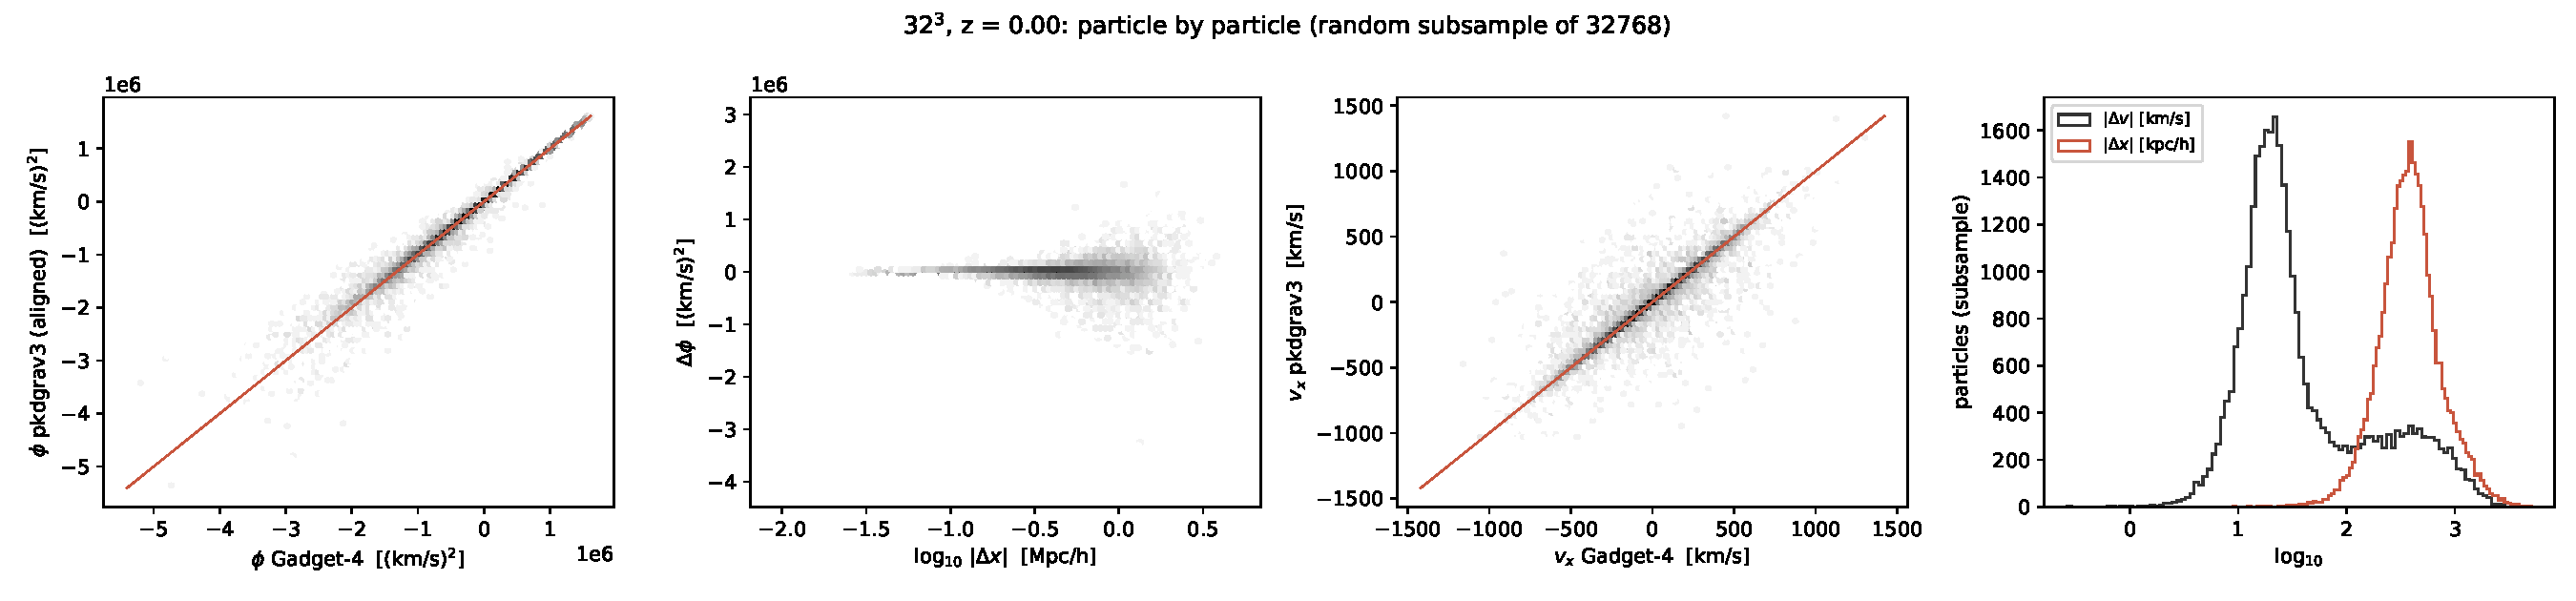
\includegraphics[width=\textwidth]{figs/particles_32_z0.pdf}
\caption{$32^3$, $z=0$, every particle: potentials (\pkd{} aligned to \gad{}'s zero point), potential difference
against particle separation, $v_x$, and the distributions of $|\Delta v|$ and $|\Delta x|$.}
\label{fig:p32}
\end{figure}

\begin{figure}[H]
\centering
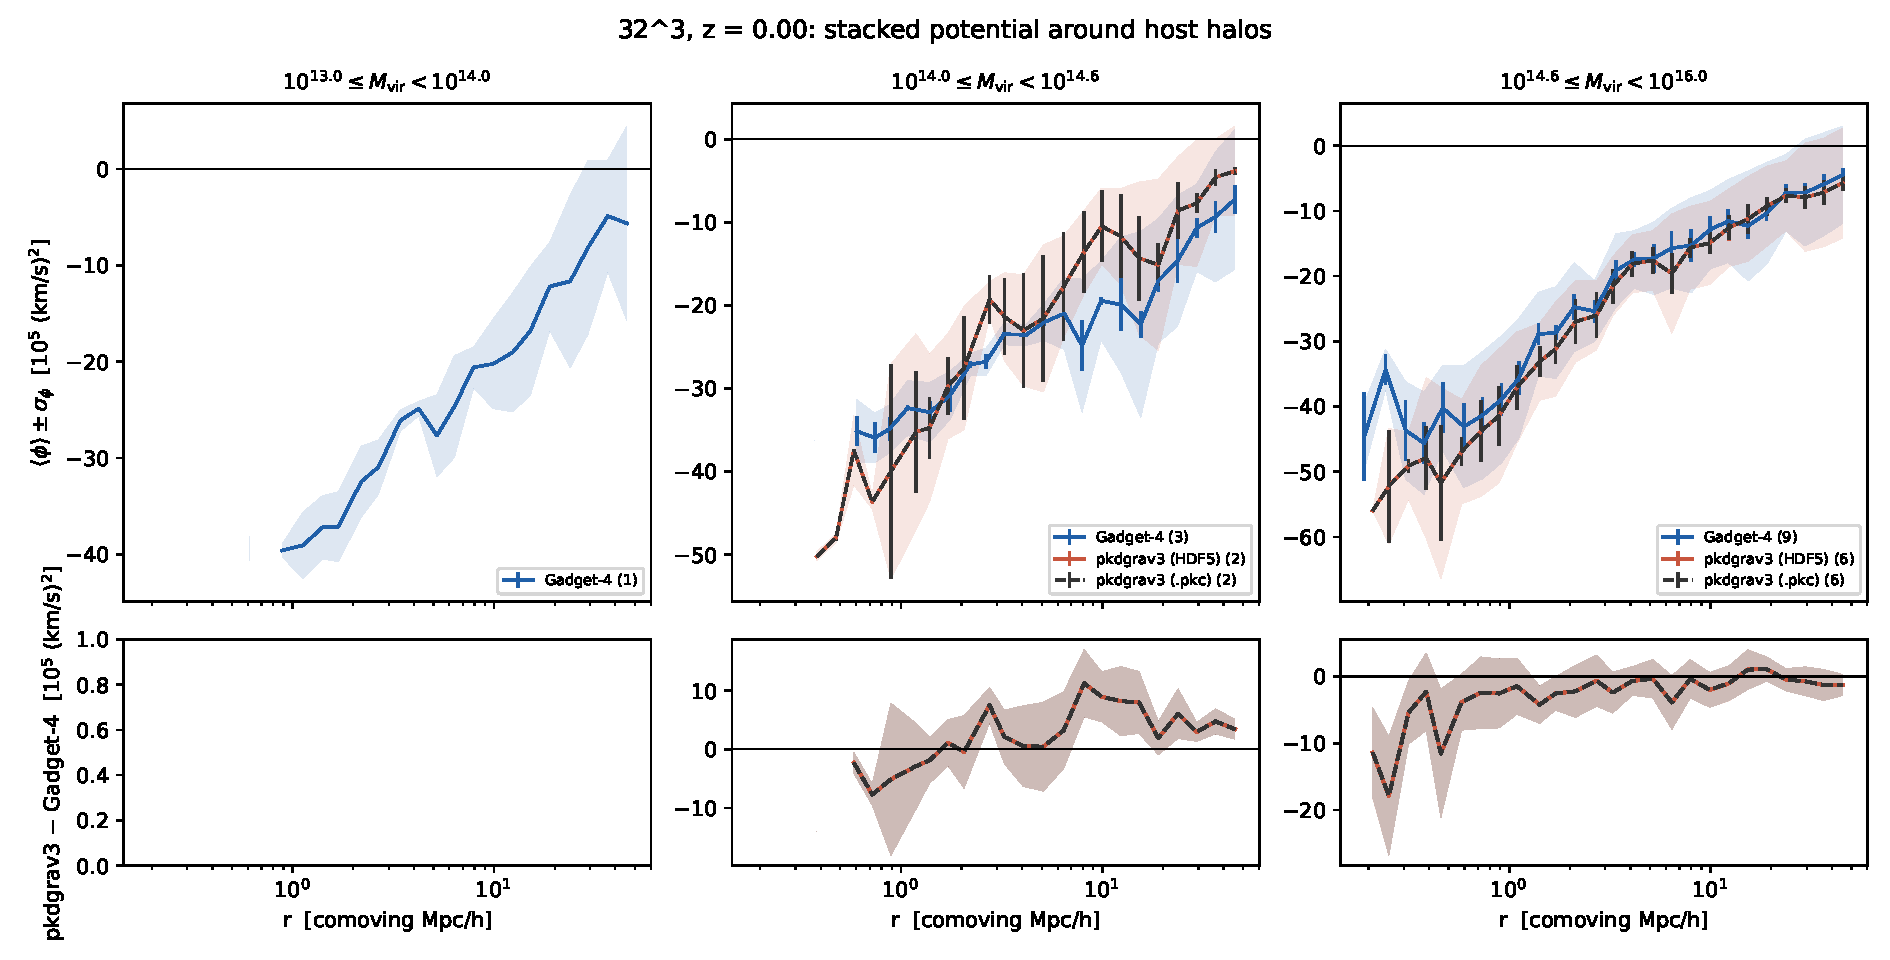
\includegraphics[width=\textwidth]{figs/stack_32_out100.pdf}
\caption{$32^3$, $z=0$: stacked potential around host halos in three $M_{\rm vir}$ bins (number of halos in the
legend). Line with error bars: mean and jackknife error; band: $\pm\sigma_\phi$, the scatter of the potential over
all pairs in the shell. Bottom: \pkd{} $-$ \gad{} (HDF5 and \texttt{.pkc} coincide).}
\label{fig:s32}
\end{figure}

The volume-weighted and linear-bin stacks were made at $32^3$ too ($64^3$ grid, spacing 3.1\,\Mpch). With 1--12
halos per bin and 0.2\,\Mpch{} shells, almost every linear shell has fewer than 50 pairs and is masked. They are in
\fp{data/pkd32_vs_gadget32_r1/profiles} and the notebook, but carry no information beyond the $256^3$ results.

\begin{figure}[H]
\centering
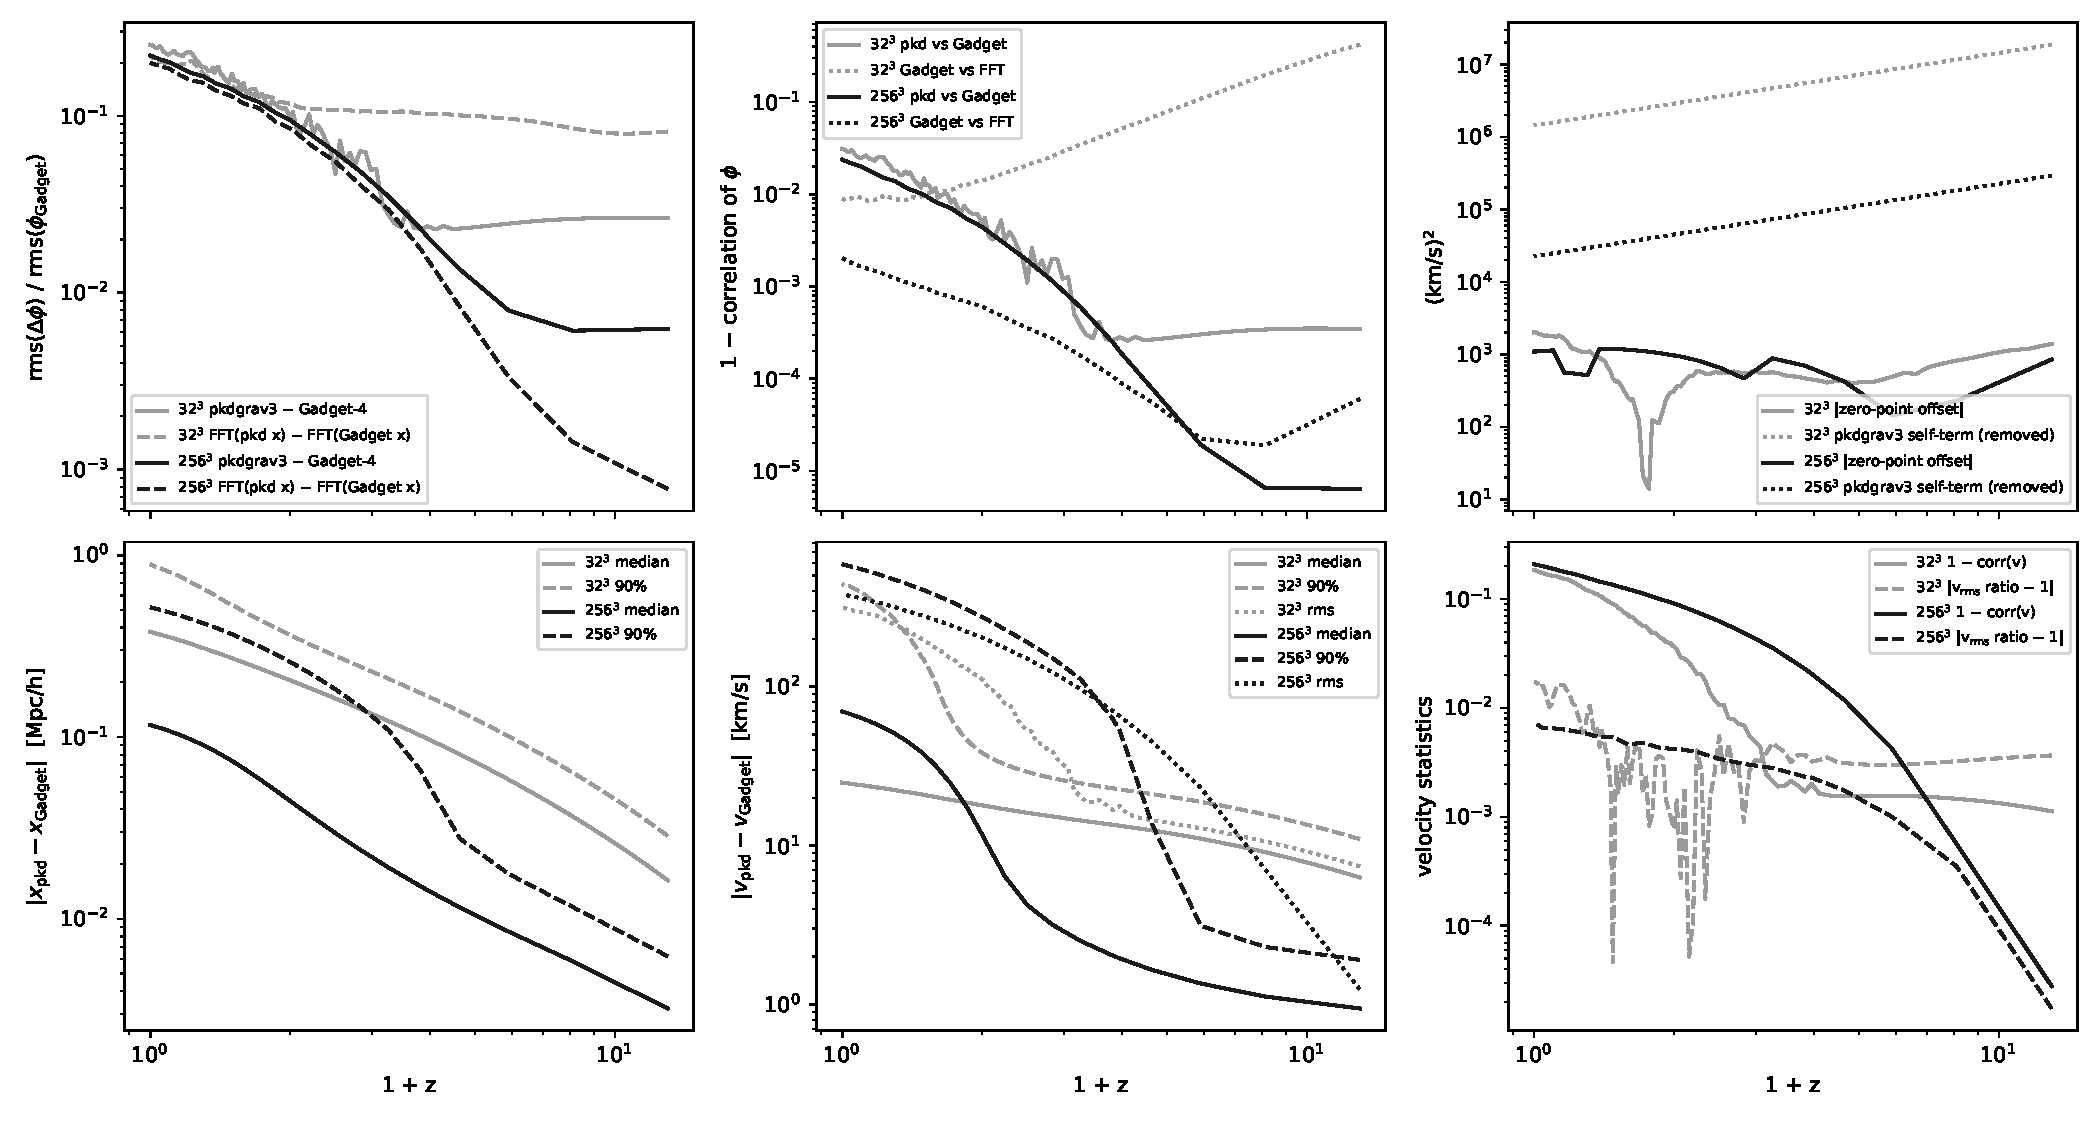
\includegraphics[width=\textwidth]{figs/particles_vs_z.pdf}
\caption{Particle-by-particle statistics against redshift (grey: $32^3$, black: $256^3$).
Top: rms potential difference over rms potential (solid) and the same for the FFT potentials of the two codes'
particle positions (dashed); $1-$correlation of the potentials; zero-point offset and \pkd{}'s removed self-term.
Bottom: particle separation, velocity difference, velocity correlation and rms-velocity ratio.}
\label{fig:pvz}
\end{figure}

\begin{figure}[H]
\centering
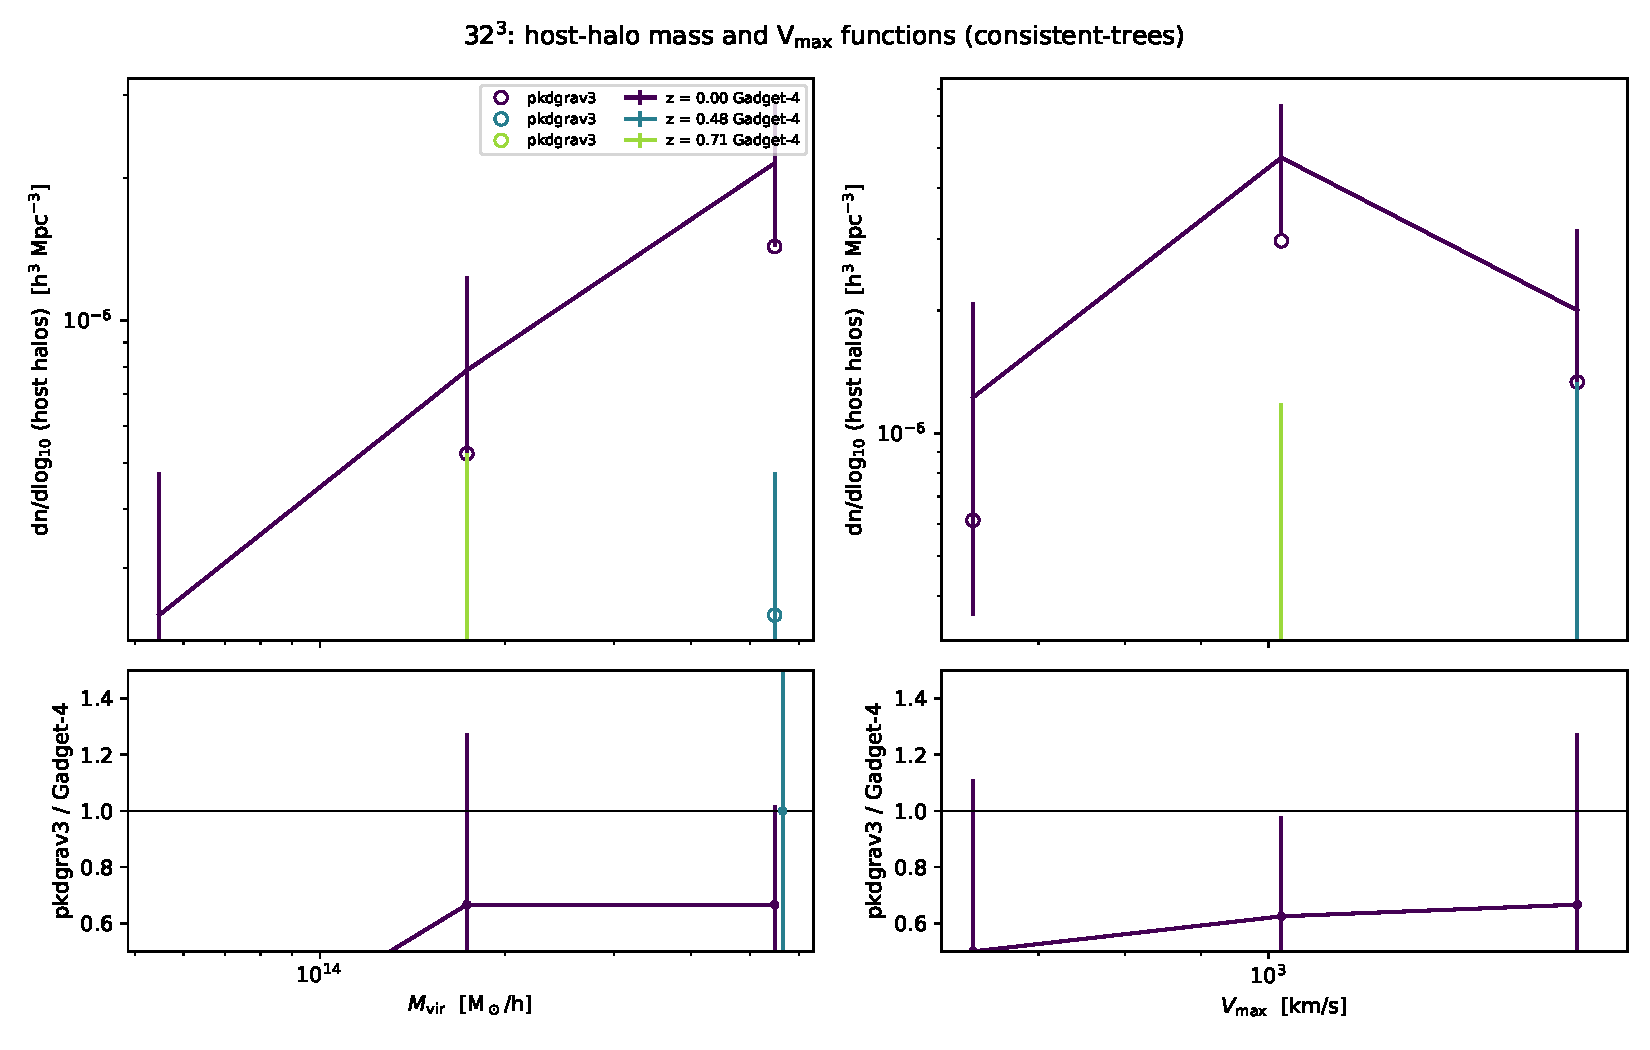
\includegraphics[width=0.75\textwidth]{figs/halo_mf_32.pdf}
\caption{$32^3$: host-halo $M_{\rm vir}$ and $V_{\max}$ functions (Rockstar) of both codes; with $\le15$ halos
per snapshot this is only a test of the tool.}
\label{fig:mf32}
\end{figure}


%======================================================================================================
\section{Results at $256^3$}
\label{sec:r256}

The $256^3$ run has particle mass $4.15\times10^{10}$\,\Msunh{}, $\epsilon_G = 26$\,$h^{-1}$kpc and
$\epsilon_P = 13$\,$h^{-1}$kpc. Both runs and the full halo pipeline completed (Table~\ref{tab:run256}).

\begin{table}[H]
\centering\small
\begin{tabular}{@{}lll@{}}
\toprule
stage & \gad{} & \pkd{} \\
\midrule
simulation & 2.9\,h, 64 MPI ranks, 101 snapshots, 63\,GB & 2.6\,h, 64 threads, 101 outputs, peak memory 14\,GB \\
Rockstar & 29\,min, 40\,658 halos at $z=0$ & 29\,min, 39\,883 halos at $z=0$ \\
consistent-trees & 10\,min, 94 hlists ($z \le 7.8$) & 11\,min, 94 hlists \\
VAHC (grid $512^3$) & 2.3\,h with 8 processes (peak 168\,GB) & 3.5\,h with 8 processes \\
comparison & \multicolumn{2}{l}{29\,min (23 outputs, peak 9\,GB); stacks 3--13\,s per code and output} \\
\bottomrule
\end{tabular}
\caption{$256^3$ jobs on pawna. consistent-trees skips the 7 earliest catalogues ($<20000$ bytes, production
threshold), so at $z > 7.8$ the halo comparison uses the Rockstar catalogues.}
\label{tab:run256}
\end{table}

\subsection{Particles: potential, positions, velocities}

\begin{table}[H]
\centering\small
\begin{tabular}{@{}rrcccccccc@{}}
\toprule
out & $z$ & corr$(\phi)$ & $\frac{{\rm rms}\,\Delta\phi}{{\rm rms}\,\phi}$ & FFT$_{x}$ & offset & med $|\Delta x|$ & 90\% $|\Delta x|$ & med $|\Delta v|$ & corr$(v)$ \\
 & & & & & \kms & \Mpch & \Mpch & km\,s$^{-1}$ & \\
\midrule
0 & 11.98 & 0.999994 & 0.006 & 0.001 & $+849$ & 0.0032 & 0.006 & 0.9 & 1.0000 \\
19 & 2.96 & 0.999802 & 0.021 & 0.015 & $-640$ & 0.014 & 0.055 & 2.0 & 0.979 \\
46 & 1.00 & 0.995549 & 0.095 & 0.085 & $-966$ & 0.045 & 0.259 & 11.9 & 0.908 \\
64 & 0.50 & 0.990111 & 0.142 & 0.129 & $-1192$ & 0.074 & 0.367 & 37.5 & 0.867 \\
100 & 0.00 & 0.976212 & 0.220 & 0.199 & $-1093$ & 0.116 & 0.517 & 69.8 & 0.791 \\
\bottomrule
\end{tabular}
\caption{$256^3$, particle by particle (columns as in Table~\ref{tab:p32}). \pkd{}'s removed self-term is
$-2.9\times10^5$\,\kms{} at $z=12$ and $-2.25\times10^4$ at $z=0$.}
\label{tab:p256}
\end{table}

\begin{itemize}
\item \textbf{Before structure forms the two codes agree very closely.} At $z=12$ the potentials correlate to
$1-6\times10^{-6}$ with 0.6\% rms difference. That is better than either code agrees with the FFT
reference ($1-6\times10^{-5}$), so it is limited by the reference, not by the codes. Particles are 3\,$h^{-1}$kpc
apart (0.12\,$\epsilon_G$) and velocities agree to 0.9\,km\,s$^{-1}$.
\item \textbf{The difference then grows with nonlinear structure}, to 2\% rms at $z = 3$, 10\% at $z=1$ and 22\% at
$z=0$ (25\% at $32^3$). From $z\approx3$ on, 75--90\% of it is accounted for by the particles being in different
places: the FFT potentials of the two sets of positions differ by 0.73 (at $z=3$) to 0.90 (at $z=0$) of the rms
$\Delta\phi$ (Fig.~\ref{fig:pvz}). The force solvers themselves agree far better than the rms suggests (see also the matched
halos below).
\item \textbf{The zero points agree} to $\le 1.2\times10^3$\,\kms{} after removing \pkd{}'s self-term, about 0.1\%
of rms $\phi$. The \texttt{.pkc} potential matches \pkd{}'s HDF5 to 0.5\,\kms{} (half the quantisation step) at
every output.
\item \textbf{Positions and velocities.} At $z=0$ the median particle separation is 0.116\,\Mpch{} (4.5
$\epsilon_G$; 15\% of the mean interparticle spacing) and the 90th percentile 0.52\,\Mpch. Velocities split into two
populations (Fig.~\ref{fig:p256}):
  \begin{itemize}
  \item particles outside halos, $|\Delta v| \approx 3$\,km\,s$^{-1}$;
  \item particles inside halos, whose orbits are chaotic, $|\Delta v| \sim 100$--300\,km\,s$^{-1}$.
  \end{itemize}
  The median is 70\,km\,s$^{-1}$ and the rms 380\,km\,s$^{-1}$. The rms velocities of the two runs differ by 0.7\% at
$z=0$.
\end{itemize}

\begin{figure}[H]
\centering
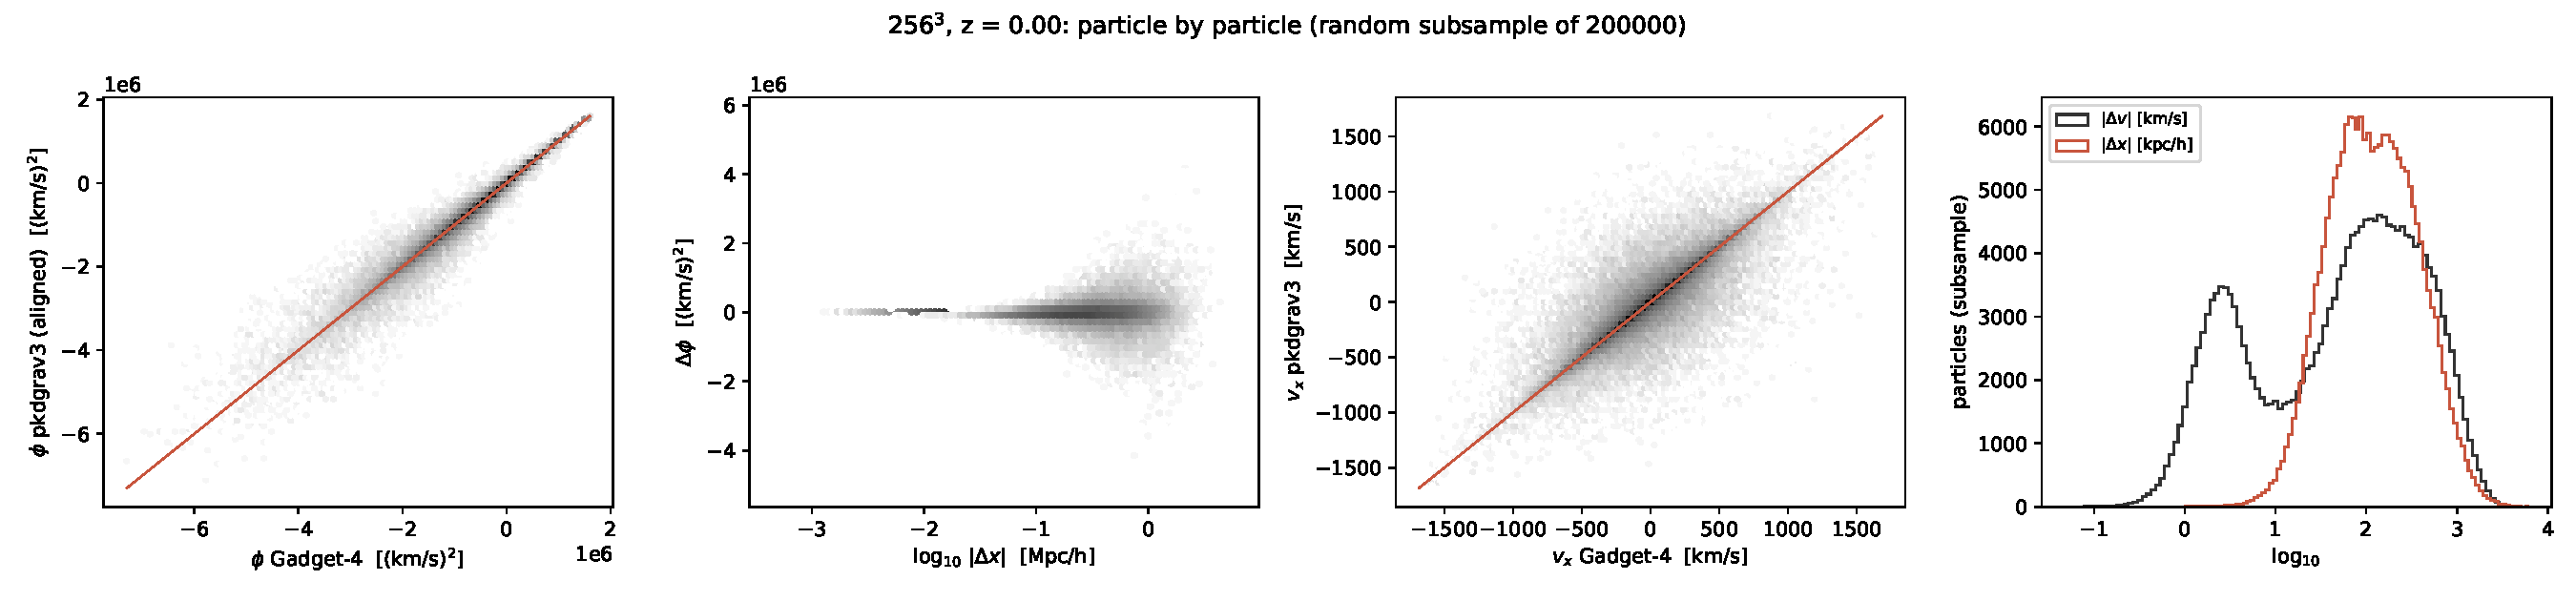
\includegraphics[width=\textwidth]{figs/particles_256_z0.pdf}
\caption{$256^3$, $z=0$, a random 200\,000 particles: potentials, $\Delta\phi$ against separation, $v_x$, and the
distributions of $|\Delta v|$ and $|\Delta x|$. The bimodal $|\Delta v|$ separates field particles from halo
particles.}
\label{fig:p256}
\end{figure}

\subsection{Halo catalogues and VAHC}

At $z=0$ there are 36\,043 (\gad{}) and 35\,404 (\pkd{}) host halos; 28\,484 are matched one to one.
\begin{itemize}
\item \textbf{Mass function} (Fig.~\ref{fig:mf256}). The $M_{\rm vir}$ functions agree within 2--3\% (and within
Poisson errors) from $10^{12}$ to $10^{14.5}$\,\Msunh{} at every redshift. Below $\sim 10^{12}$\,\Msunh{} (30
particles) \pkd{} has 5\% fewer halos at $5\times10^{11}$ and 13\% fewer at $2\times10^{11}$.
\item \textbf{The $V_{\max}$ function differs more.} \pkd{} has 14--17\% fewer halos at 100--160\,km\,s$^{-1}$ and
13--19\% more at 300--600\,km\,s$^{-1}$ ($z=0$; about half as much at $z=1$). This follows from the halo structure
below.
\item \textbf{Matched halos} (Fig.~\ref{fig:match256}). The matched fraction is $\ge 96\%$ above
$3\times10^{12}$\,\Msunh{}, 79\% at $10^{12}$--$3\times10^{12}$ and 45\% at
$3\times10^{11}$--$10^{12}$.
  \begin{itemize}
  \item \emph{Masses} agree: median ratio 1.00 above $10^{12}$\,\Msunh{}, with 16--84\% range $\pm12\%$ at $10^{12}$
  narrowing to $\pm2\%$ at $10^{14}$.
  \item \emph{\pkd{} halos are more concentrated}: $R_{\rm vir}/r_s$ is higher by 21--26\% at
  $10^{12}$--$10^{13}$\,\Msunh{}, 9\% at $3\times10^{13}$ and 3\% above $10^{14}$. Their $V_{\max}$ is 2--5\% higher.
  \item \emph{Shapes}: above $3\times10^{12}$\,\Msunh{} \pkd{} halos are somewhat rounder, with $c/a$ higher by 6--17\%.
  \item \emph{Spin} agrees (median ratio 0.99--1.02).
  \item \emph{Centres and bulk velocities}: the median centre offset is 0.24\,$R_{\rm vir}$ at $10^{12}$, 0.11 at
  $10^{13}$ and 0.03 at $3\times10^{14}$\,\Msunh{}. Bulk velocities differ by 15--80\,km\,s$^{-1}$ (median).
  \end{itemize}
  The higher central density is consistent with \pkd{}'s smaller effective softening ($2\epsilon_P = \epsilon_G$
  against \gad{}'s spline support $2.8\epsilon_G$). It is largest at $10^{12}$--$10^{13}$\,\Msunh{}, where
  $r_s$ is only a few $\epsilon_G$.
\item \textbf{VAHC.} The halo-by-halo bias $b_1$ is measured from the density field at $k<0.1\,h$\,Mpc$^{-1}$, which
the two runs share. It is identical (correlation 1.0000; rms difference 0.010, against a halo-to-halo scatter of 3.4).
The tidal eigenvalue $\lambda_1$ correlates at 0.98 with $R = 4R_{200b}$ smoothing (rms difference 1.0, scatter 5.4)
and at 0.94 with $2R_{200b}$, where the halo's own surroundings, which differ in detail, matter more.
\item \textbf{Potential of matched halos} (Fig.~\ref{fig:hpot256}).
  \begin{itemize}
  \item \pkd{}'s $\phi_{\min}$ is 4--9\% deeper (median per mass decade at $z=0$), the mean potential of the 10\% most
  bound particles 4--6\% deeper, and $\langle\phi\rangle$ within $R_{\rm vir}$ 1--2\% deeper. This is the same
  central-density difference.
  \item For the same particles, \pkd{}'s mean potential of each \gad{} halo's members agrees with \gad{}'s to
  0.1--0.5\%. That is the cleanest test of the two potentials, free of halo-finder and centring differences.
  \end{itemize}
\end{itemize}

\begin{figure}[H]
\centering
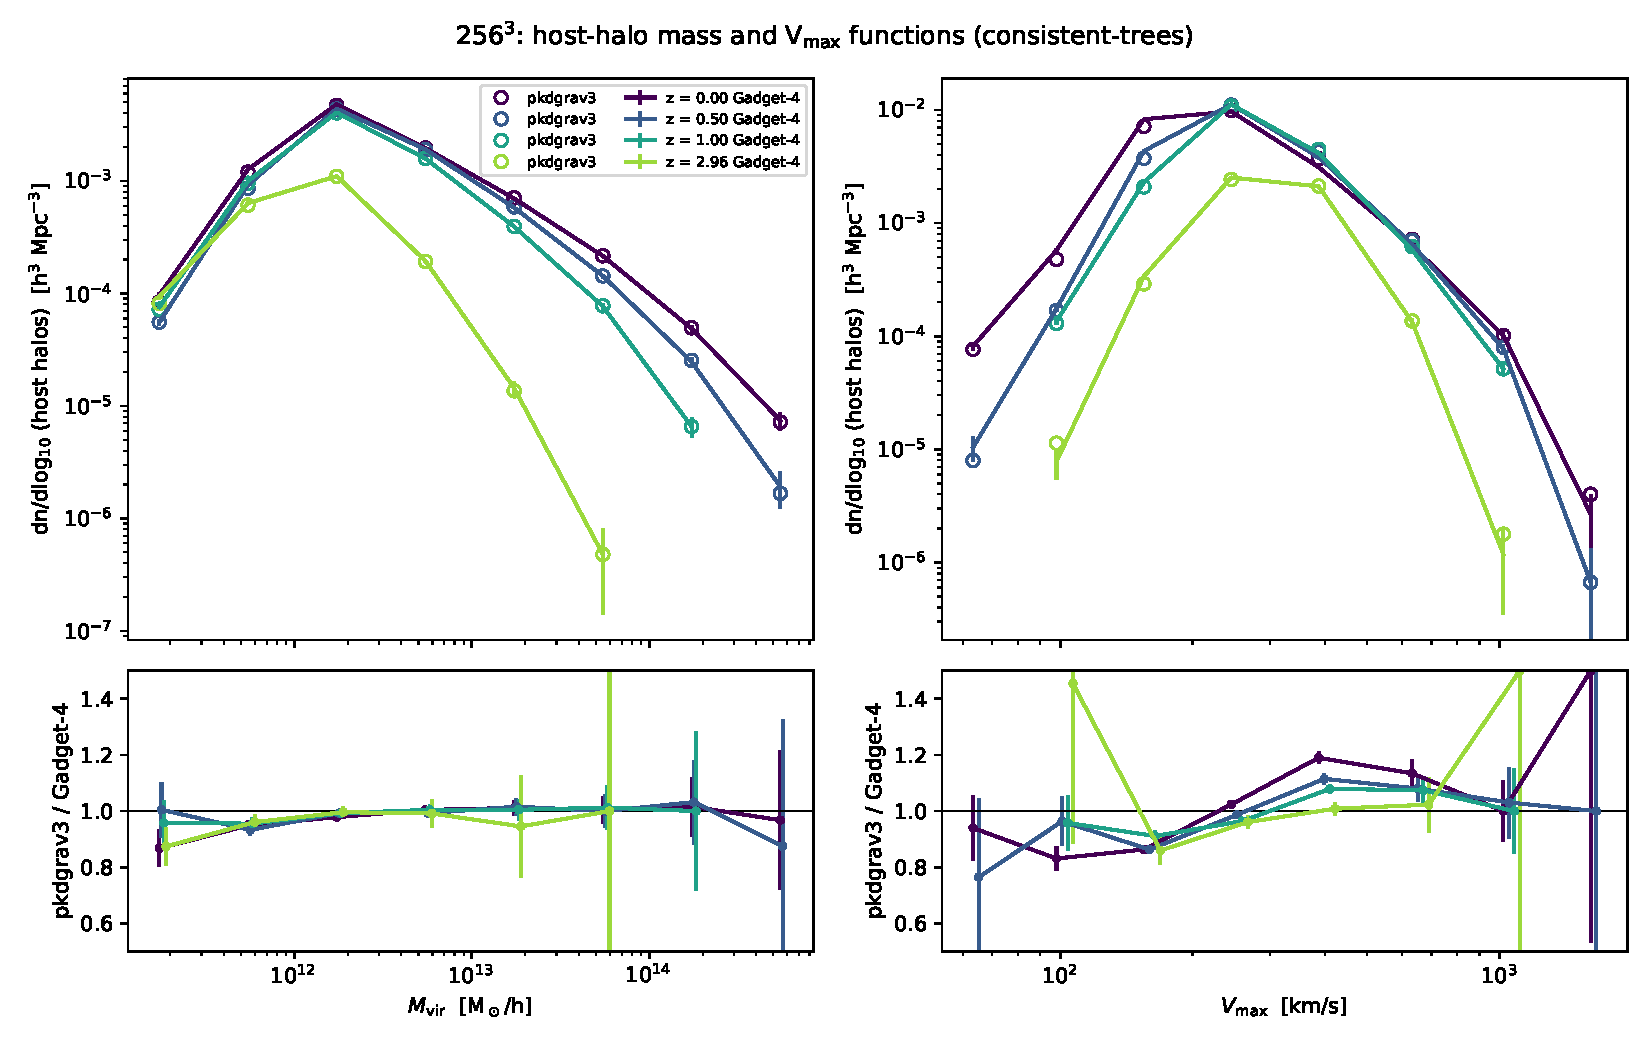
\includegraphics[width=0.85\textwidth]{figs/halo_mf_256.pdf}
\caption{$256^3$: host-halo $M_{\rm vir}$ and $V_{\max}$ functions from the consistent-trees catalogues of the two
codes at $z\approx3$, 1, 0.5 and 0 (lines with errors: \gad{}; circles: \pkd{}). Bottom: ratio with Poisson errors.}
\label{fig:mf256}
\end{figure}

\begin{figure}[H]
\centering
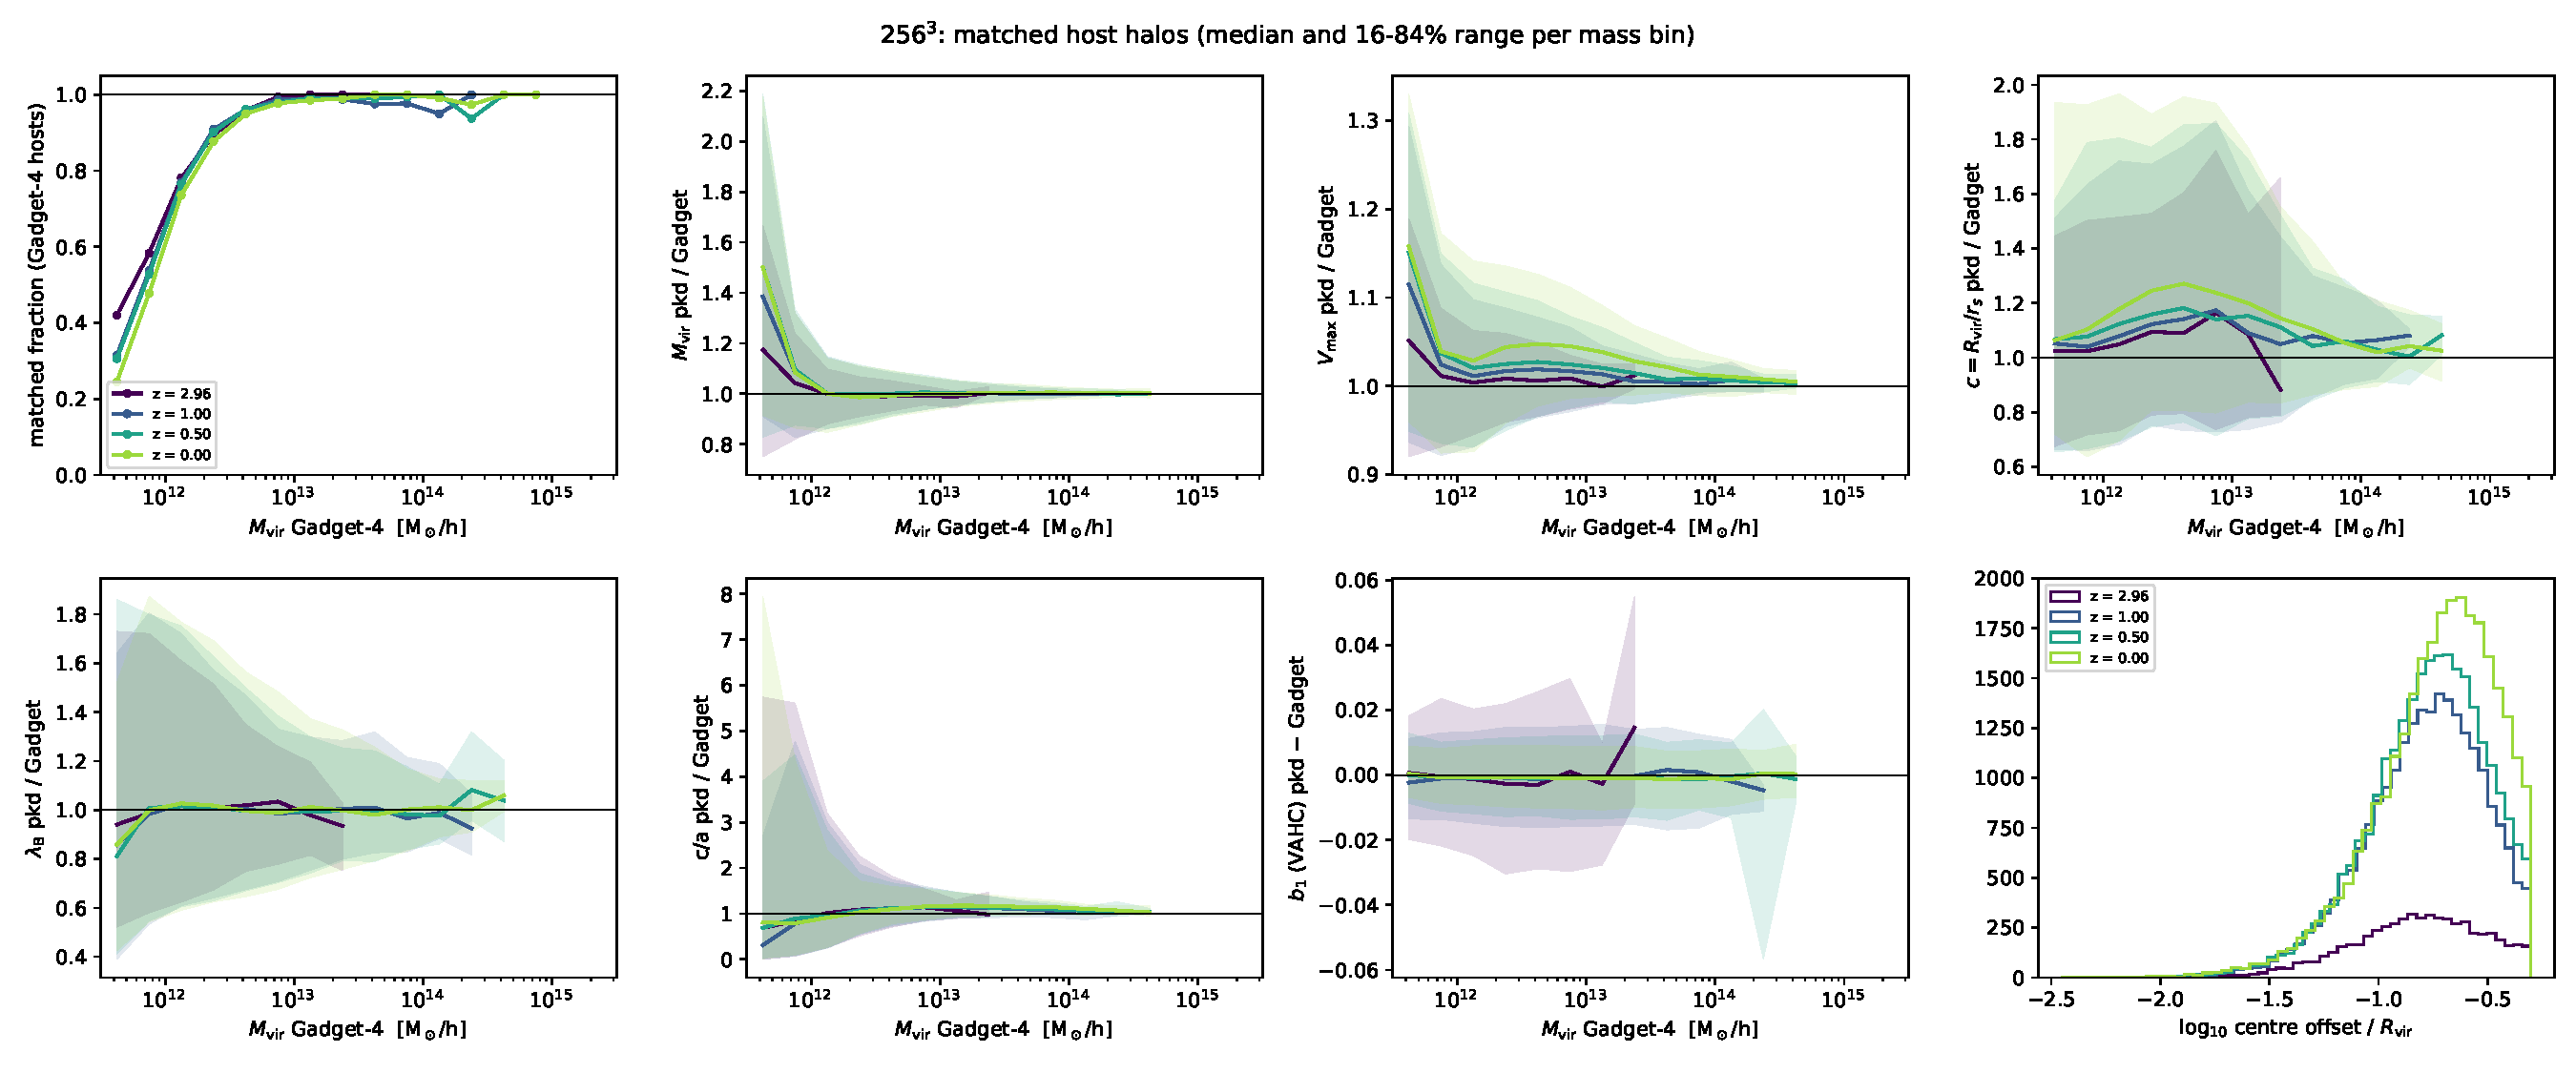
\includegraphics[width=\textwidth]{figs/halo_match_256.pdf}
\caption{$256^3$: matched host halos. Matched fraction, and per \gad{} mass bin the median (line) and 16--84\% range
(band) of \pkd{}/\gad{} for $M_{\rm vir}$, $V_{\max}$, concentration, spin and $c/a$; the difference of the VAHC
bias $b_1$; and the distribution of centre offsets.}
\label{fig:match256}
\end{figure}

\begin{figure}[H]
\centering
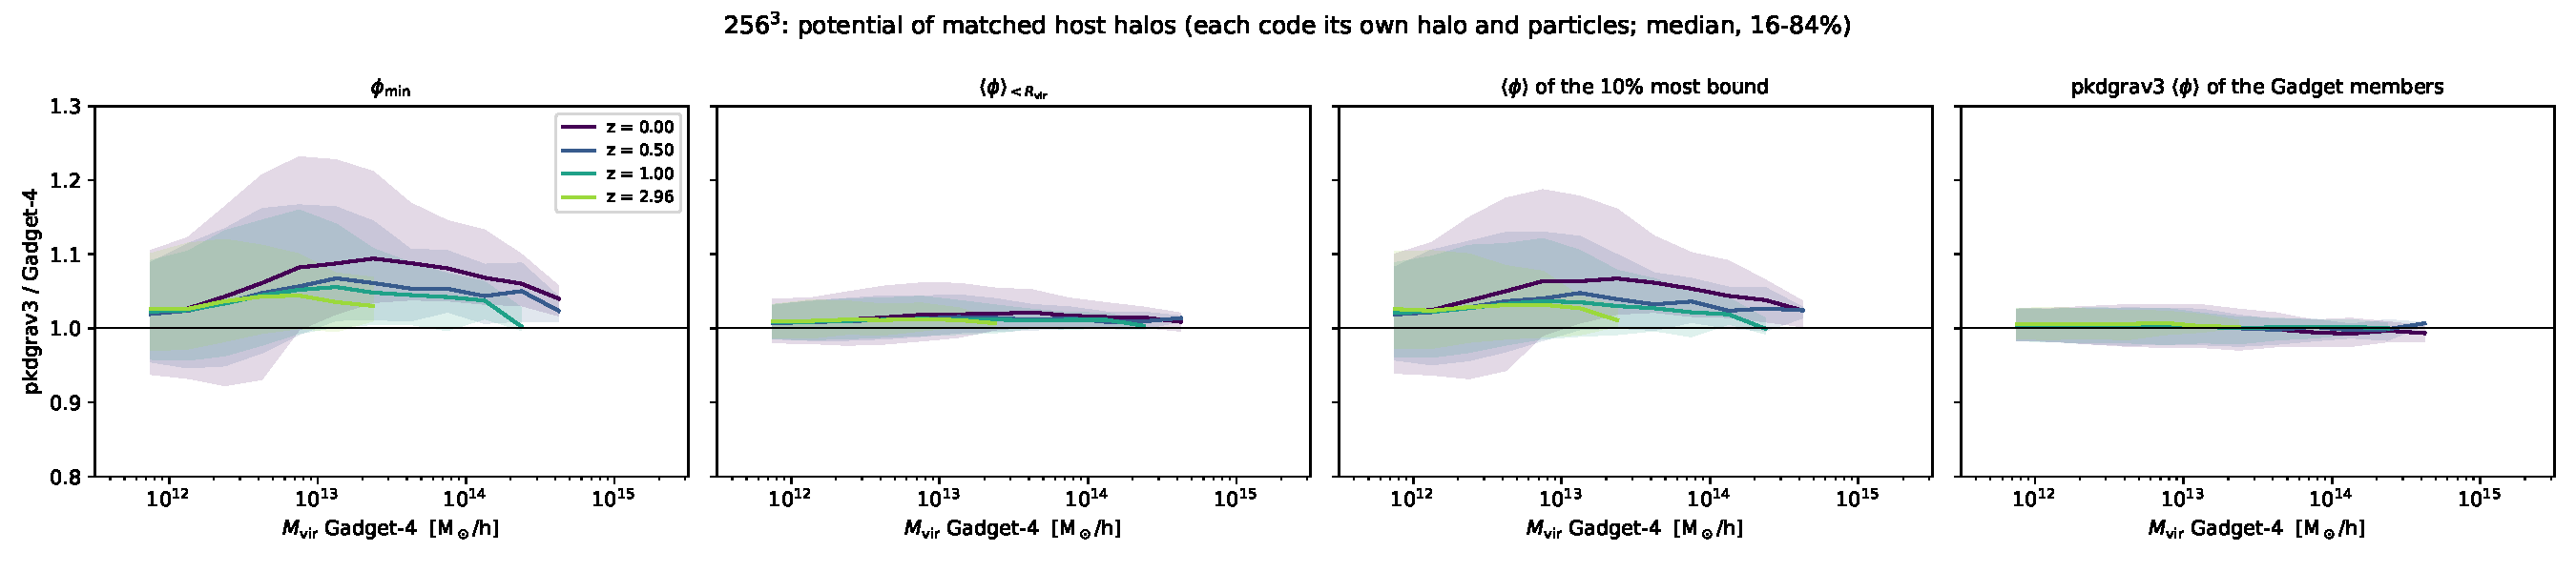
\includegraphics[width=\textwidth]{figs/halo_potential_256.pdf}
\caption{$256^3$: potential of matched host halos, \pkd{}/\gad{}. Each code uses its own halo and its own particles
within $R_{\rm vir}$, except in the last panel, where \pkd{}'s potential is evaluated for the \gad{} halo's member
particles (same IDs).}
\label{fig:hpot256}
\end{figure}

\subsection{Stacked potential around halos}

Figures~\ref{fig:s256}--\ref{fig:xi256} come from the notebook \fp{stack_potential.ipynb}. Each code uses its own
host halos in four $M_{\rm vir}$ bins. At $z=0$ these hold 13\,375 / 3\,181 / 525 / 78 halos in \gad{}
($2\times10^{12}$--$10^{13}$, $10^{13}$--$5\times10^{13}$, $5\times10^{13}$--$2\times10^{14}$, $>2\times10^{14}$\,\Msunh)
and the same within 1\% in \pkd{}. Differences carry the paired jackknife error: the two codes' differences
over the same sub-cubes, which removes the shared large-scale (sample) variance. The dilution uses the same particle
IDs in both codes, so the subsampling noise of the outer shells cancels as well.

\begin{itemize}
\item \textbf{Shape.} $\langle\phi\rangle(r)$ is deepest at the centre, from $-5\times10^{5}$\,\kms{} in the lowest
bin to $-5\times10^6$ in the highest. In the low-mass bins it has a second minimum at 1--3\,\Mpch: small halos
often sit near larger ones. It is still $\approx -6\times10^5$\,\kms{} at 50\,\Mpch, because halos live in
large-scale potential wells. The scatter $\sigma_\phi$ in a shell, $(5$--$10)\times10^5$\,\kms, is set by the
large-scale potential and is much larger than any code difference.
\item \textbf{\pkd{} $-$ \gad{}.}
  \begin{itemize}
  \item Inside $\sim0.1$\,\Mpch{} \pkd{} is deeper: by 3--5\% at 0.05\,\Mpch{} (3--6 paired errors), and by up to
  $3\times10^5$\,\kms{} (6\%) at 0.02\,\Mpch{} in the most massive bin. This is the softening and concentration
  difference.
  \item From 0.2 to 50\,\Mpch{} the mean potentials agree to 1--2\% (mostly within 2 paired errors) at all four
  redshifts. In units of the shell scatter that is $|\Delta\langle\phi\rangle| \le 0.02\,\sigma_\phi$.
  \end{itemize}
\item \textbf{\texttt{.pkc} = HDF5.} \pkd{}'s compressed snapshots give the same stacks as its HDF5 snapshots at all
radii.
\item \textbf{Matter around the halos} (Fig.~\ref{fig:xi256}). $1+\xi_{hm}$ agrees within 2\% beyond 0.1\,\Mpch.
Inside, \pkd{} has more mass: +50\% at 0.02\,\Mpch{} in the lowest bin, falling to $\lesssim 10\%$ in the
highest.
\end{itemize}

\begin{figure}[H]
\centering
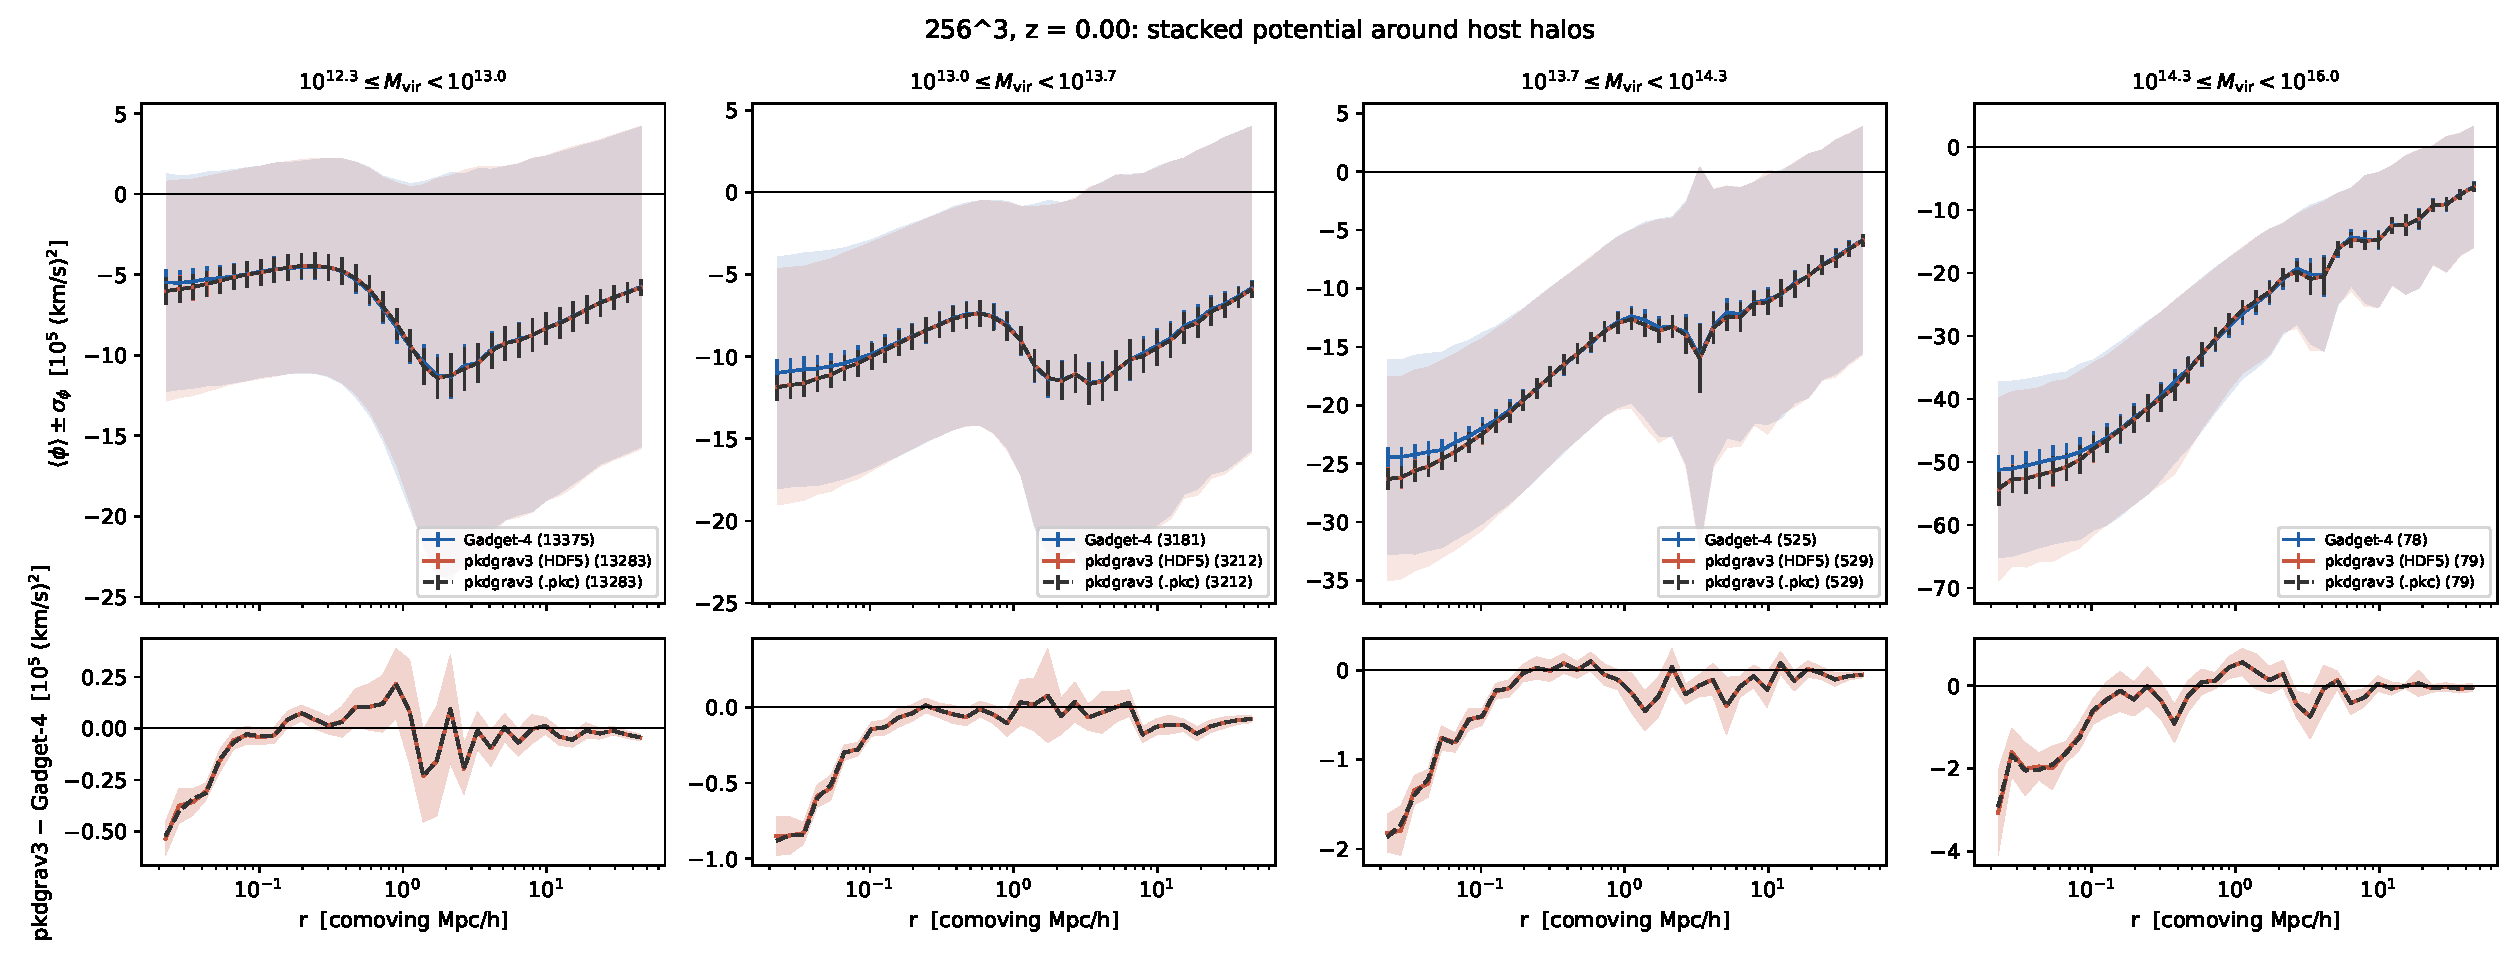
\includegraphics[width=\textwidth]{figs/stack_256_out100.pdf}
\caption{$256^3$, $z=0$: stacked potential around host halos in four $M_{\rm vir}$ bins out to 50\,\Mpch{} (number of
halos in the legend). Lines with error bars: mean and jackknife error; bands: $\pm\sigma_\phi$. Bottom: \pkd{} $-$
\gad{} (solid: HDF5, dashed: \texttt{.pkc}) with the paired jackknife error.}
\label{fig:s256}
\end{figure}

\begin{figure}[H]
\centering
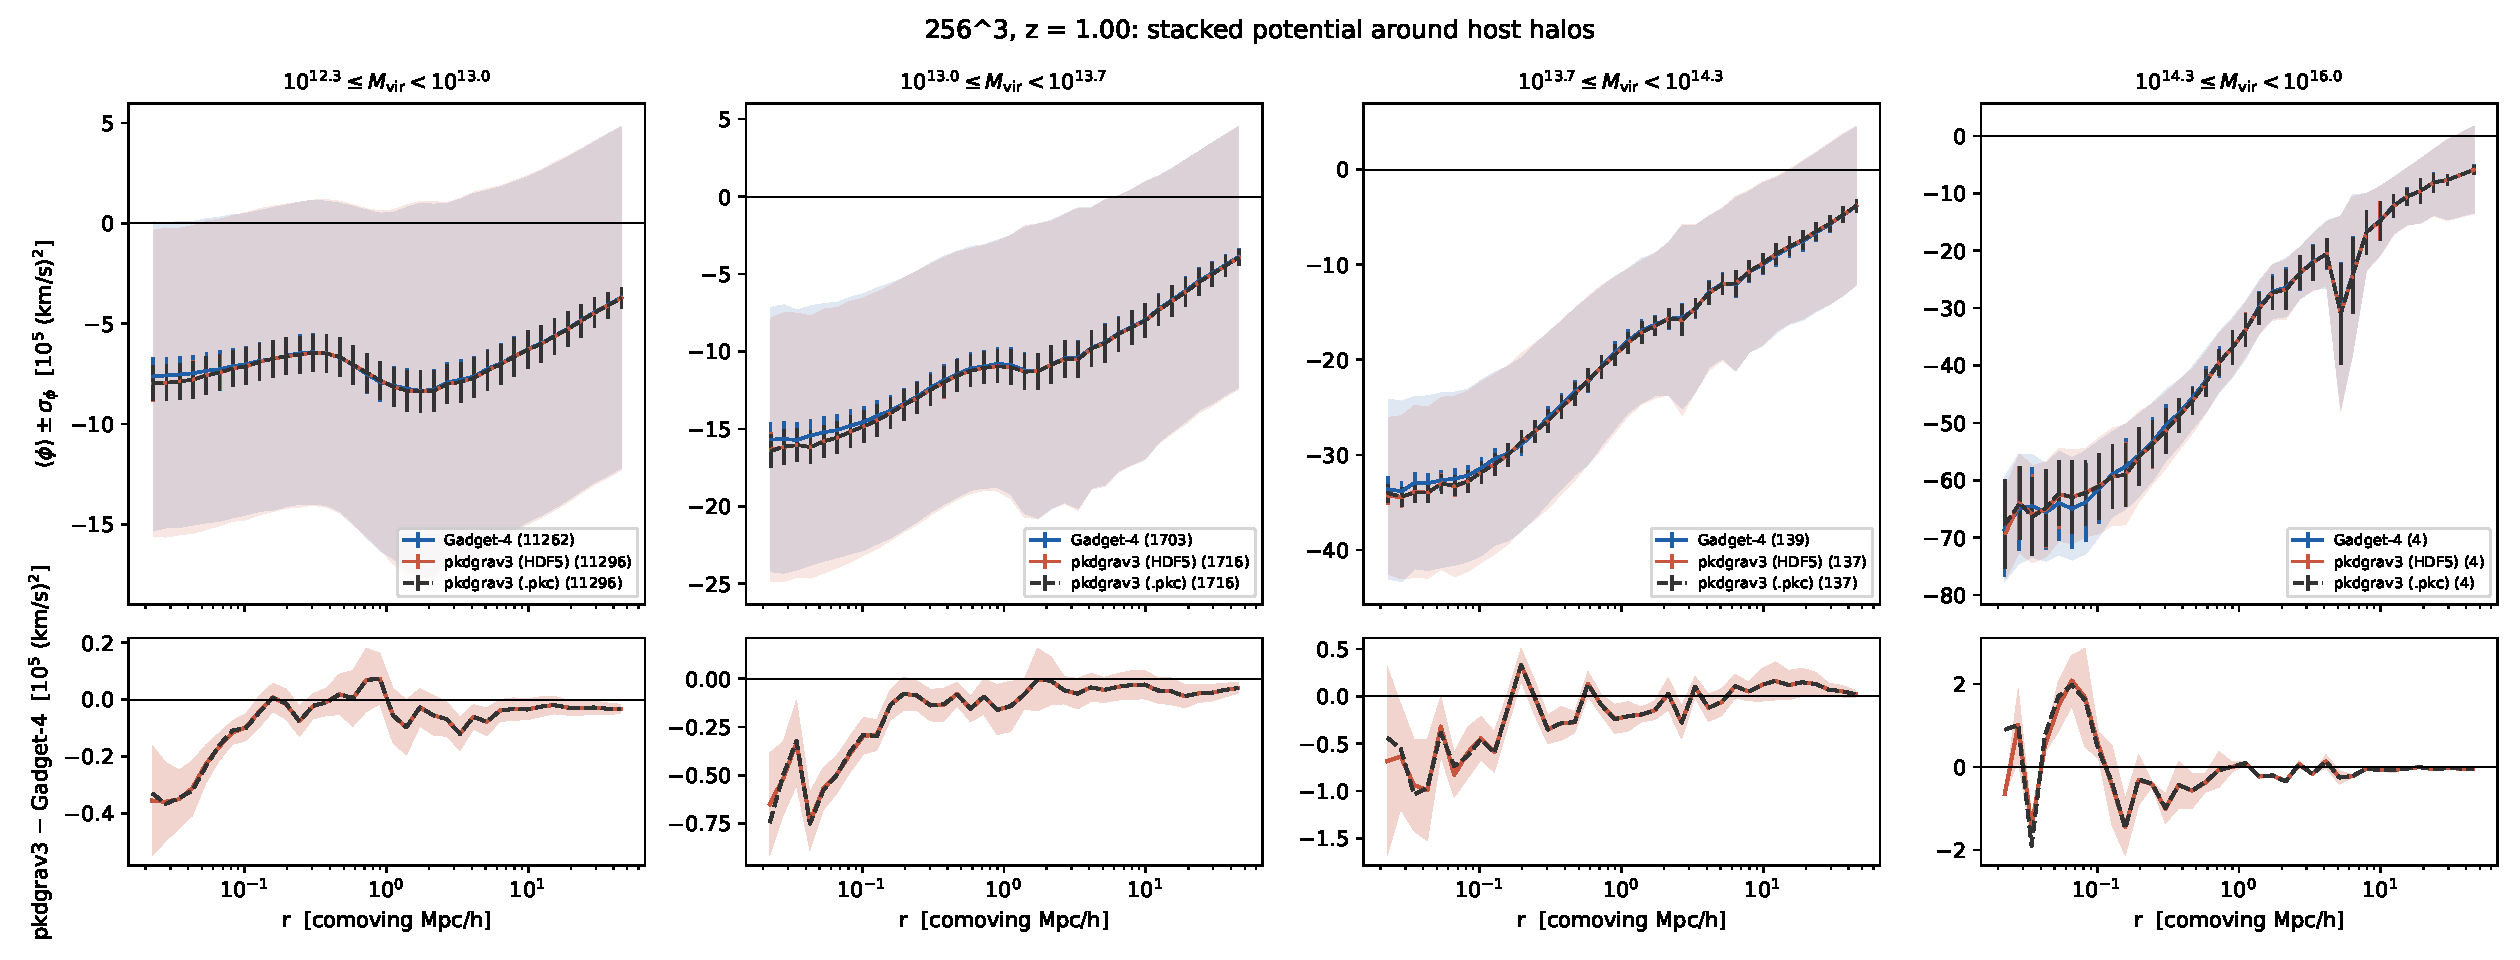
\includegraphics[width=\textwidth]{figs/stack_256_out046.pdf}
\caption{As Fig.~\ref{fig:s256} at $z = 1$.}
\end{figure}

\begin{figure}[H]
\centering
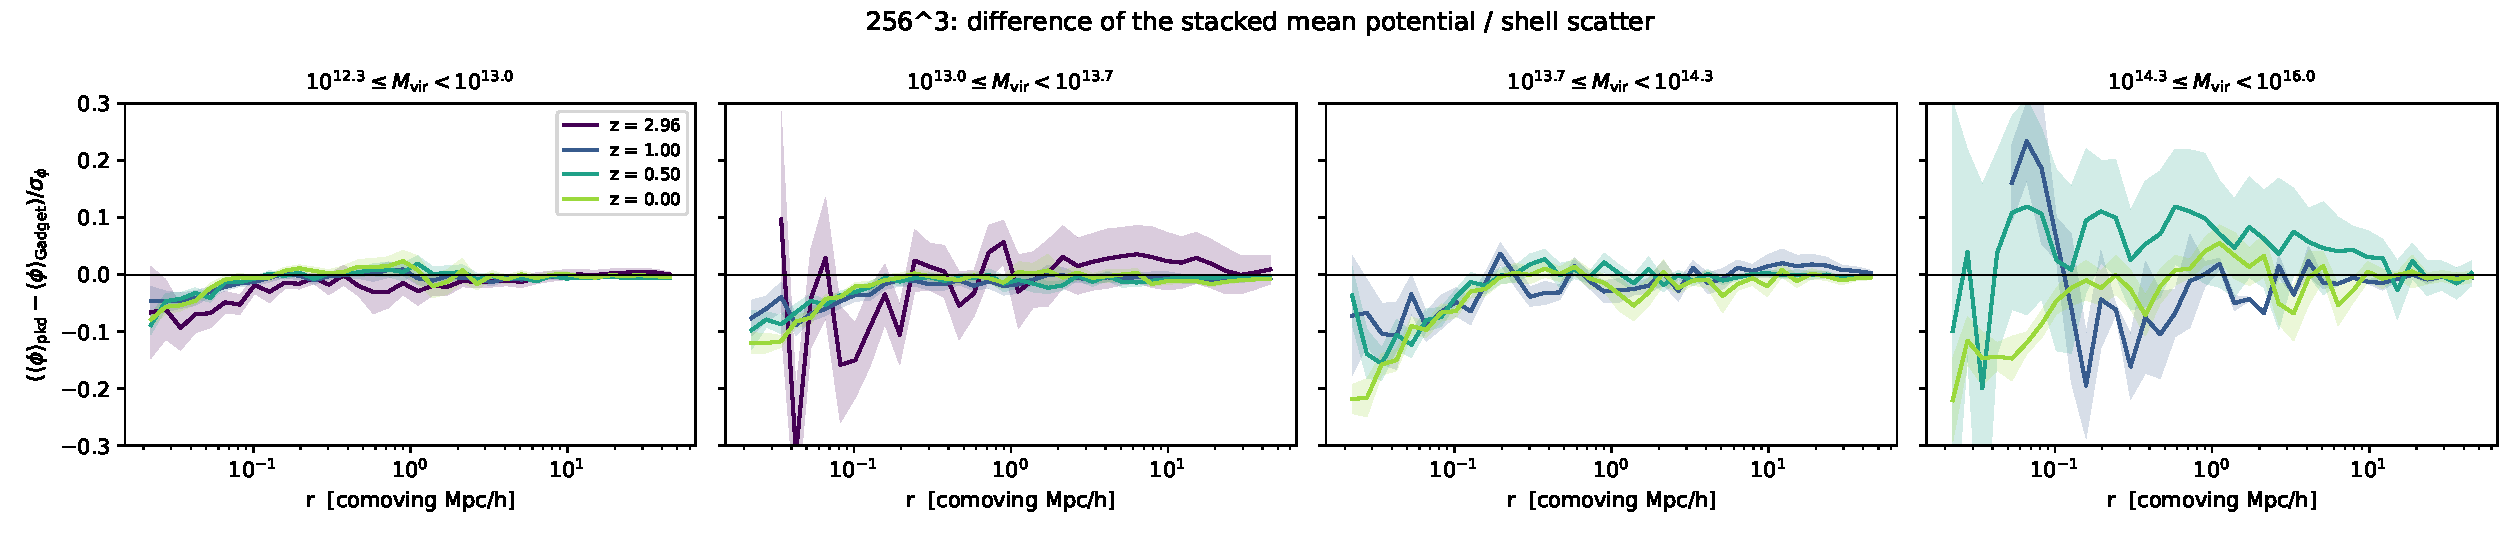
\includegraphics[width=\textwidth]{figs/stack_rel_256.pdf}
\caption{$256^3$: $\Delta\langle\phi\rangle/\sigma_\phi$ at $z \approx 3$, 1, 0.5 and 0, with the paired jackknife
error.}
\label{fig:srel256}
\end{figure}

\begin{figure}[H]
\centering
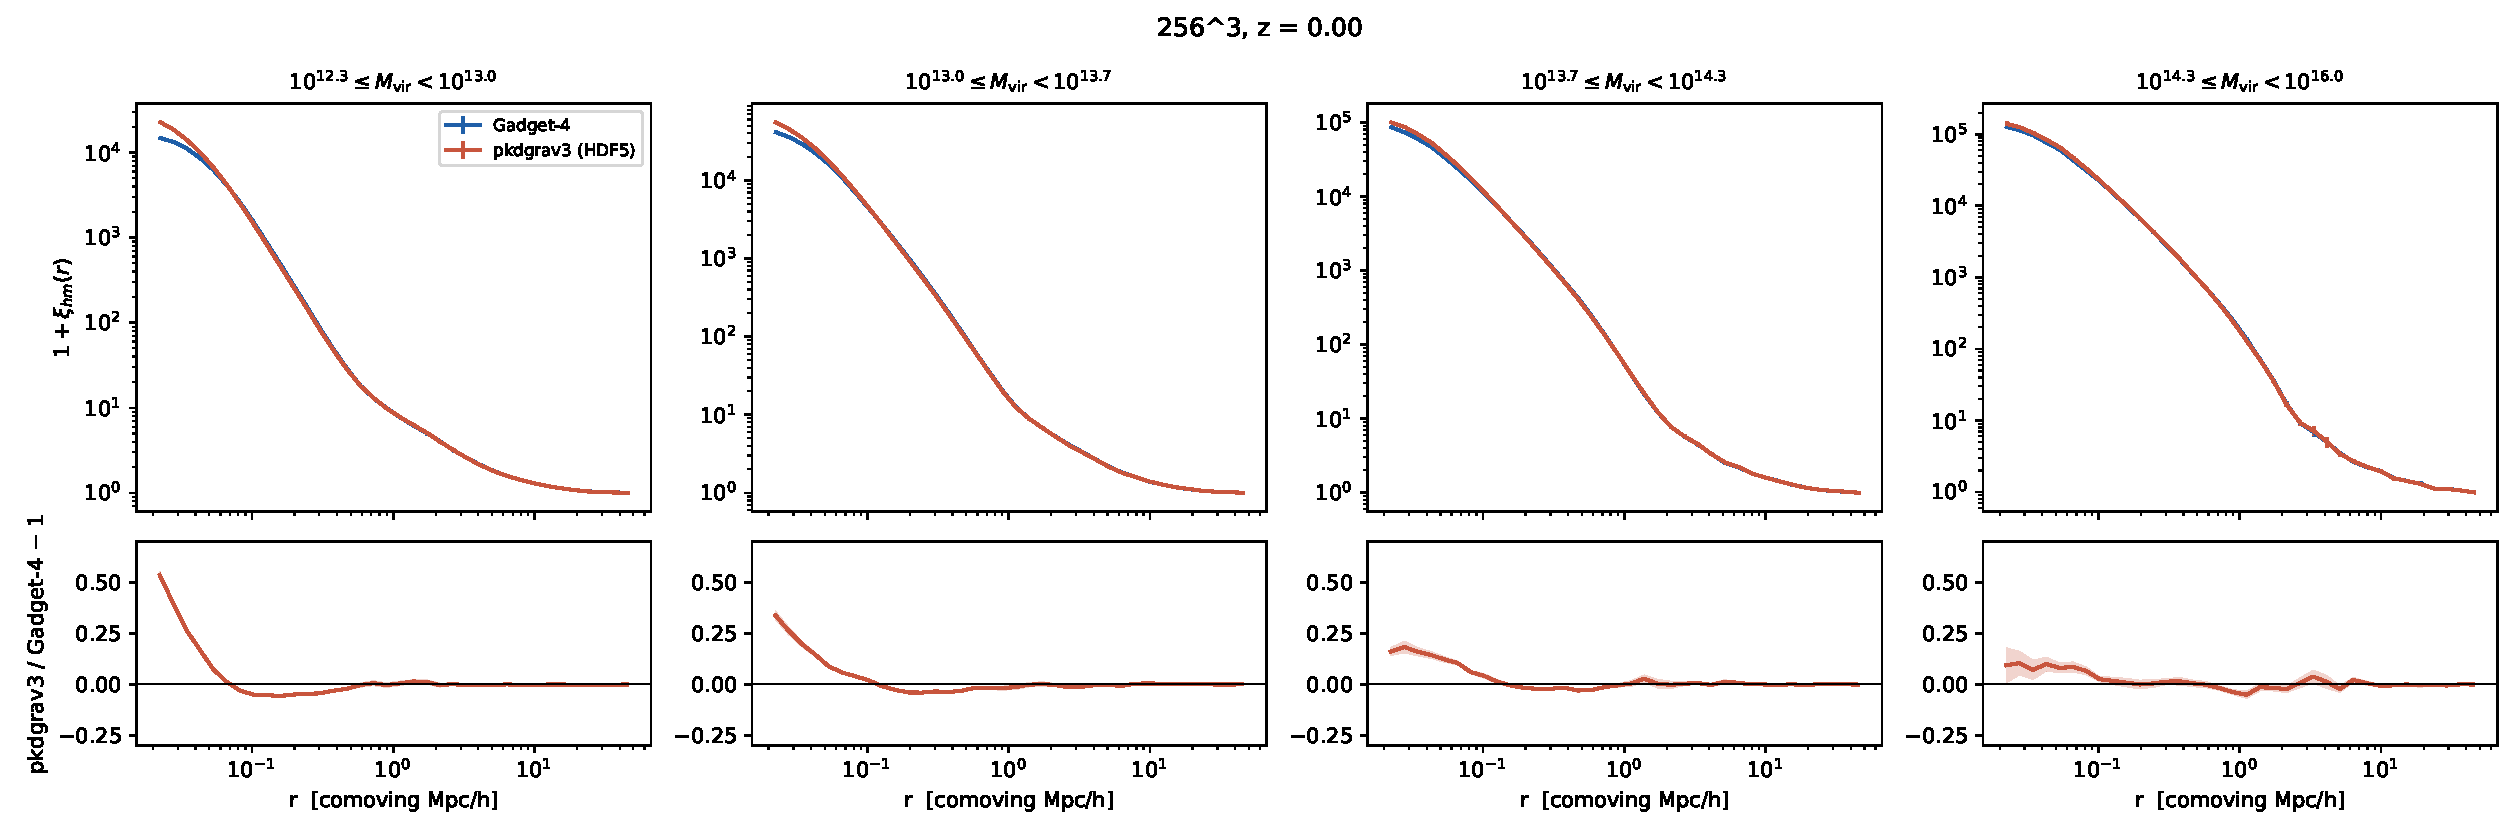
\includegraphics[width=\textwidth]{figs/xihm_256.pdf}
\caption{$256^3$, $z=0$: halo--matter cross-correlation from the same stacks; bottom: \pkd{}/\gad{} $-1$ with the
paired jackknife error.}
\label{fig:xi256}
\end{figure}


%======================================================================================================
\section{Problems found on the way}
\label{sec:issues}
\begin{enumerate}
\item \textbf{\gad{} writes Potential $=0$ without \texttt{EVALPOTENTIAL}.} The first $32^3$ run, with the exact
production Config (\texttt{OUTPUT\_POTENTIAL} only), has zero potential everywhere
(\fp{data_run1_zeropot/}). The production Sahyadri Config lacks \texttt{EVALPOTENTIAL}, so the production
\gad{} snapshots most likely have no potential (not checked directly). Adding the flag left the ICs and output
times byte-identical.
\item \textbf{consistent-trees needs many halos per snapshot}: it fails at $32^3$ (``too few halos at scale factor
0.768278 to calculate consistency metric'') even after relaxing \fp{gen_merger_cfg.pl}'s 20000-byte catalogue
threshold. At $256^3$ the production threshold is used.
\item \textbf{VAHC is the slowest stage at $256^3$}: 20--40\,min per snapshot and process at grid $512^3$ (FFT
smoothing at many scales and per-halo loops), $\sim$23\,GB per process. With 4 processes, 94 snapshots did not fit in
10\,h; the jobs were rerun with 8 processes and 30\,h (restartable: finished snapshots are skipped). At $2048^3$
with 100 outputs this stage needs planning.
\item \textbf{Column names}: consistent-trees hlists call the columns \texttt{Mvir}, \texttt{Rvir}; Rockstar lists
\texttt{ID}, \texttt{X}, \ldots. The comparison scripts read both (fixed during the $256^3$ run; the first two
comparison jobs stopped on this).
\item \textbf{\pkd{} has no physical units when it reads an IC file} (\fp{units.cxx}): box size in the output
headers and \texttt{.pkc} potential units are wrong unless \fp{dKpcUnit} and \fp{dMsolUnit} are given; the
pipeline's parameter generator now writes them. A Gadget-2 input file's IDs become iOrder directly, so they must be
$0\ldots N-1$; \pkd{}'s HDF5 \texttt{Header/Time} is code time, not $a$. Recorded in the \pkd{} fork,
\fp{docs/compressed_io_plan.md} section 7.
\end{enumerate}

%======================================================================================================
\section{Reproducing}
\begin{verbatim}
# on pawna, in a clone of sahyadri-sandbox (branch gadget-pkdgrav3-potential)
cd scripts/gadget_pkdgrav3_compare
bash -lc "bash setup_gadget4_pawna.sh <gadget4 source> <G4HOME> 256"   # Gadget-4 builds (once)
bash submit_compare.sh compare256.conf                                 # 9 PBS jobs
# figures (Mac or anywhere with matplotlib), from reports/gadget_pkdgrav3_potential:
rsync pawna:<data>/compare/pkd256_vs_gadget256_r1/{particles.csv,profiles,halos} data/pkd256_vs_gadget256_r1/
jupyter nbconvert --to notebook --execute stack_potential.ipynb
python make_figures.py 32=data/pkd32_vs_gadget32_r1 256=<copy with snap_*.npz>
latexmk -pdf report.tex
\end{verbatim}

\end{document}
